% 可自定义论文时间戳 \today
% \year=2021
% \month=5
% \day=20

\documentclass{sysuthesis} % 默认使用电子版(不填充空白页)。如果需要双面打印版,请注释掉本行并启用下一行
% \documentclass[print-both-sides]{sysuthesis} % 使用双面打印版(填充额外空白页以保证每一章开头都在奇数页)
\usepackage{minted}  % 在论文中使用代码
\usepackage{multirow}
\usepackage{booktabs}
%%
% 论文相关信息
% 本文档中前缀"c-"代表中文版字段, 前缀"e-"代表英文版字段
% modifyer: 黄俊杰(huangjj27, 349373001dc@gmail.com)
% update date: 2017-04-13
%%

% 标题
% 论文题目应以简短、明确的词语恰当概括整个论文的核心内容,避免使用不常见的缩略词、缩写字。读者通过标题可大致了解毕业设计(论文)的内容、专业的特点和科学的范畴。中文题目一般不宜超过 24 个字,必要时可增加副标题。外文题目一般不宜超过 12 个实词

% 封面标题。由于技术所限,封面题目过长的划分交由用户您进行定夺
% 这也能让您的论文封面看起来更有美感
\covertitlefirst{基于 POD 降阶模型的}
\covertitlesecond{流场重构方法研究}

% Author:   Souler Ou
% 修改者:    欧一锋
% Date:     3/30/2018
% Mail:     ou@souler.cc
%如果英文标题过长可以使用此两项作为表三(答辩记录表)的标题。
\etitlefirst{}
\etitlesecond{}

% 中文标题
\ctitle{中山大学本科毕业论文}
\etitle{ }

% 作者详细信息
\author{王慧心}
\cauthor{王\ 慧\ 心}    % 封面作者
\eauthor{Wang Huixin}
\studentid{21310234}
\cschool{系统科学与工程学院}

\cmajor{信息工程}
\emajor{Computer Science and Technology}

% 指导老师
\cmentor{段焰辉 \ (副教授)}
\ementor{Prof.段焰辉 }

     % 论文相关信息
%%
% 开题报告
% modifier: 黄俊杰(huangjj27, 349373001dc@gmail.com)
% update date: 2017-05-14

% 选题目的
\objective{

}

% 思路
\methodology{

}

% 研究方法/程序/步骤
\researchProcedure{

}

% 相关支持条件
\supportment{

}

% 进度安排
\schedule{

}

% 指导老师意见
\proposalInstructions{

}

   % 开题报告内容
%%
% 摘要信息
% 本文档中前缀"c-"代表中文版字段, 前缀"e-"代表英文版字段
% 摘要内容应概括地反映出本论文的主要内容,主要说明本论文的研究目的、内容、方法、成果和结论。要突出本论文的创造性成果或新见解,不要与引言相 混淆。语言力求精练、准确,以 300—500 字为宜。
% 在摘要的下方另起一行,注明本文的关键词(3—5 个)。关键词是供检索用的主题词条,应采用能覆盖论文主要内容的通用技术词条(参照相应的技术术语 标准)。按词条的外延层次排列(外延大的排在前面)。摘要与关键词应在同一页。
% modifier: 黄俊杰(huangjj27, 349373001dc@gmail.com)
% update date: 2017-04-15
%%

\cabstract{
本研究旨在解决航空航天等领域流场特性分析中传统计算流体力学(CFD)方法计算成本高、效率低的问题,提出了一种创新的基于本征正交分解(POD)降阶模型的流场重构方法。从希尔伯特空间变分原理出发,建立基于 Snapshot POD 的自适应基函数生成框架,大幅降低流场维度。结合三次样条插值技术,构建完整的 POD 降阶模型(POD-ROM)流场重构框架,有效解决非采样工况下的模态耦合问题。进一步引入克里金(Kriging)预测方法,提升模型对复杂流场的预测能力。以 NACA0012 翼型为研究对象,运用专业 CFD 软件模拟生成多工况流场数据,对所提方法进行验证。数值实验结果表明,该方法在保证最大相对误差不超过 5\% 的前提下,计算效率较传统 CFD 方法提升了两个数量级。研究成果为无人机防除冰系统设计、气动性能优化等工程应用提供了有力的技术支撑,同时在计算效率和预测精度方面展现出显著优势,具有重要的工程应用价值。
}
% 中文关键词(每个关键词之间用“,”分开,最后一个关键词不打标点符号。)
\ckeywords{本征正交分解;降阶模型;流场重构;NACA0012 翼型;三次样条插值;计算流体力学;克里金模型}
\eabstract{
    This study aims to address the issues of high computational cost and low efficiency of traditional computational fluid dynamics (CFD) methods in the analysis of flow field characteristics in aerospace and other fields. An innovative flow field reconstruction method based on the proper orthogonal decomposition (POD) reduced-order model is proposed. Starting from the variational principle in Hilbert space, an adaptive basis function generation framework based on Snapshot POD is established, which greatly reduces the dimension of the flow field. By combining with the cubic spline interpolation technique, a complete flow field reconstruction framework of the POD reduced-order model (POD-ROM) is constructed, effectively solving the modal coupling problem under non-sampled conditions. Furthermore, the Kriging prediction method is introduced to improve the model's prediction ability for complex flow fields. Taking the NACA0012 airfoil as the research object, professional CFD software is used to simulate and generate flow field data under multiple working conditions to verify the proposed method. The results of numerical experiments show that this method can ensure that the maximum relative error does not exceed 5\%, and the computational efficiency is increased by two orders of magnitude compared with traditional CFD methods. The research results provide strong technical support for engineering applications such as UAV anti-icing system design and aerodynamic performance optimization. At the same time, it shows significant advantages in computational efficiency and prediction accuracy, and has important engineering application value.
}
% 英文文关键词(每个关键词之间用,分开, 最后一个关键词不打标点符号。)
\ekeywords{Proper Orthogonal Decomposition; Reduced-Order Modeling; Flow Field Reconstruction; NACA0012 Airfoil; Cubic Spline Interpolation; Computational Fluid Dynamics; Kriging Model}

     % 摘要内容
%%
% 成绩评定记录表
% modifier: 黄俊杰(huangjj27, 349373001dc@gmail.com)
% update date: 2017-05-17

\gradingComment{
    某某同学针对什么问题研究了什么算法/实现了什么系统/针对这个系统做了什么测试,本文选题合理,实验结果表明技术路线……论文写作规范,引用文献充分,符合中山大学本科论文的规范,是篇优秀/良好/中等/合格的论文。
}
    % 成绩评定记录表评语
%%
% 四次进度报告相关信息

% Author:   Souler Ou
% 修改者:    欧一锋
% Date:     3/30/2018
% Mail:     ou@souler.cc

% 第一次进度报告
\firstsummary{
	\begin{adjustwidth}{2em}{2em}
		在这一阶段,XXX工作基本完成,主要在如下几个方面:
		\begin{enumerate}
			\item 完成了第一项。
			\item 完成了第二项
			\item 完成了第三项。
		\end{enumerate}
	\end{adjustwidth}
}
% 第2次进度报告
\secondsummary{
	\begin{adjustwidth}{2em}{2em}
		...
	\end{adjustwidth}
}
% 第3次进度报告
\thirdsummary{
	\begin{adjustwidth}{2em}{2em}
		...
	\end{adjustwidth}
}
% 第4次进度报告
\fourthsummary{
	\begin{adjustwidth}{2em}{2em}
		...
	\end{adjustwidth}
}
% 第1次老师评价
\firstcomment{
	\begin{adjustwidth}{2em}{2em}
		论文完成情况良好。
	\end{adjustwidth}
}
% 第2次老师评价
\secondcomment{
	\begin{adjustwidth}{2em}{2em}
		...
	\end{adjustwidth}
}
% 第3次老师评价
\thirdcomment{
	\begin{adjustwidth}{2em}{2em}
		...
	\end{adjustwidth}
}
% 第4次老师评价
\fourthcomment{
	\begin{adjustwidth}{2em}{2em}
		...
	\end{adjustwidth}
}
% 老师总评价
\finalcomment{
	\begin{adjustwidth}{2em}{2em}
		...
	\end{adjustwidth}
}   % 过程检查报告数据
\begin{document}
% 论文前置部分
\frontmatter
\pagenumbering{Roman}
\makeUndergraduateCover    % 封面
\makeUndergraduateTitlePage    % 扉页
% \makeProposal% 开题报告
% \makeProgressCheck  % 过程检查记录表
% \makeDefenseRecord  % 答辩情况等级表
\makedisclaim       % 学术诚信声明
\makeabstract       % 中英文摘要
\maketableofcontents        % 目录
\makelistoffiguretable

% 论文主体部分
\mainmatter
% 引言

% 正文
%%
% 引言或背景
% 引言是论文正文的开端,应包括毕业论文选题的背景、目的和意义;对国内外研究现状和相关领域中已有的研究成果的简要评述;介绍本项研究工作研究设想、研究方法或实验设计、理论依据或实验基础;涉及范围和预期结果等。要求言简意赅,注意不要与摘要雷同或成为摘要的注解。
% modifier: 黄俊杰(huangjj27, 349373001dc@gmail.com)
% update date: 2017-04-15
%%
\usetikzlibrary{shapes,arrows,positioning}

\chapter{绪论}
%定义,过去的研究和现在的研究,意义,与图像分割的不同,going deeper
\label{cha:introduction}
\section{研究背景}
\label{sec:background}
% What is the problem
% why is it interesting and important
% Why is it hards, why do naive approaches fails
% why hasn't it been solved before
% what are the key components of my approach and results, also include any specific limitations,do not repeat the abstract
%contribution
在航空航天、能源动力及环境工程等领域,流场特性分析是气动设计、设备优化及流动控制的核心基础。以无人机气动外形设计为例,翼型表面压力分布、边界层分离特性及尾流涡结构的精确获取,直接影响无人机的升力效率、阻力特性及抗结冰性能。然而,传统计算流体力学(CFD)方法依赖精细化网格划分与长时间数值迭代,对 NACA0012 等典型翼型进行全工况模拟时,单工况计算耗时可达数小时至数天,难以满足工程设计中多参数快速迭代的需求。尤其在无人机防除冰设计中,需实时评估不同结冰厚度、液态水含量对翼型流场的影响,传统 CFD 方法的高计算成本成为技术瓶颈。
本征正交分解(proper orthogonal decomposition,POD)方法由 Lumley\textsuperscript{\cite{lumley1967structure}} 提出,其思想为将流场分解为若干正交的空间模态,依据模态能量大小进行排序,通过线性叠加前几阶高阶模态实现原流场的精确重构。因 POD 方法可对流场实现
时空解耦,在低速圆柱绕流\textsuperscript{\cite{wang2023}}、翼型流动\textsuperscript{\cite{sun2022analysis}} 等领域得到了推广应用。近年来,POD 方法发展为可从一系列流场“快照”矩阵中提取出本征模态,并通过模态能量占比排序采用部分模态表征流场绝大部分特征,实现原始流场的重构,已被广泛应用在非定常流场数据处理以及流动特征性分析等方面。在航空、能源等领域,流场参数的精确预测对飞行器设计、能源设备优化至关重要。\textsuperscript{\cite{HKDI202407028}}
NACA0012 翼型作为对称翼型的经典代表,其流场特性随攻角变化呈现丰富的流动现象:小攻角时为附着流动,中等攻角时出现边界层分离,大攻角时形成显著分离涡,是研究流动分离、失速特性的理想对象。然而,该翼型在跨音速流动时的激波 - 边界层干扰、结冰条件下的外形畸变对流场的影响,均需高效的流场重构方法支撑。目前,工程中仍依赖全尺寸 CFD 模拟获取流场数据,缺乏适用于多工况快速预测的高效工具。因此,构建基于 POD 的 NACA0012 翼型流场重构方法,对提升无人机气动设计效率、降低研发成本具有重要现实意义。



%%引言是论文正文的开端,应包括毕业论文选题的背景、目的和意义;对国内外研究现状和相关领域中已有的研究成果的简要评述;介绍本项研究工作研究设想、研究方法或实验设计、理论依据或实验基础;涉及范围和预期结果等。要求言简意赅,注意不要与摘要雷同或成为摘要的注解。
\section{研究目的和意义}
本研究致力于深入探究基于 POD 降阶模型的流场重构方法,重点聚焦于插值 POD 方法在翼型流场分析中的应用。研究旨在实现两大核心目标:一是显著提升流场重构的精度,使重构后的流场能够高度还原真实流场的复杂特性,包括压力分布、速度梯度以及涡量等关键物理量的准确再现\cite{Smith2020};二是大幅提高流场重构的效率,降低计算成本,缩短计算时间,满足实际工程中对快速、准确流场分析的迫切需求\cite{Jones2019}。

具体而言,本研究选取经典的 NACA0012 翼型模型作为研究对象,运用插值 POD 方法对其流场进行精确重构\cite{Lee2021}。通过与专业 CFD 软件模拟生成的真实数据进行全面、细致的对比分析,系统验证插值 POD 方法在流场重构中的有效性和准确性\cite{Wang2022}。这一研究过程不仅有助于深入理解 POD 降阶模型在流场重构中的内在作用机制,揭示其背后的数学原理和物理意义\cite{Cao2020},还能为实际工程应用提供可靠、实用的技术手段。

在实际工程应用中,准确的流场重构结果能够为翼型的优化设计提供坚实的科学依据。工程师可以根据重构后的流场信息,有针对性地调整翼型的几何参数,如翼型厚度、弯度以及前缘半径等,设计出更高效、更节能的翼型\cite{Yang2023}。例如,通过流场重构发现翼型前缘的压力集中问题,可以优化前缘形状,降低压力峰值,减少阻力,提高升阻比\cite{Zhang2018}。同时,本研究成果还可以为风力发电叶片设计\cite{Chen2021}、船舶水动力性能优化\cite{Liu2022}等相关领域提供有益的借鉴和参考,推动整个相关领域的技术创新和发展,为社会经济的可持续发展做出贡献。
\section{国内外研究现状和相关工作}
\label{sec:related_work}
\subsection{ POD 降阶模型的研究现状}
POD 方法最早由 Kosambi 于1943年提出\cite{Kosambi1943},经过多年的发展,在理论研究和实际应用方面均取得了长足进步。在理论层面,众多学者致力于改进 POD 模型,以增强其对复杂流场的适应性和重构精度。例如,为了更好地捕捉流场中的动态变化特性,研究者引入时间延迟嵌入技术\cite{Schmid2011},将时间序列中的历史信息融入 POD 分析中。通过构建时间延迟坐标系统,POD 模型能够有效提取流场中的动态特征,如涡旋的生成、演化和消散过程\cite{Rowley2009}。多尺度分析方法的引入也是理论研究的重要进展之一。该方法通过将流场分解为不同尺度的成分,分别进行 POD 分析,能够更细致地描述多尺度复杂流场的特性\cite{Lumley2017}。例如,在研究大气边界层流场时,多尺度 POD 分析可以清晰地分离出大尺度的湍流结构和小尺度的粘性耗散区域\cite{Taira2020},为深入理解大气边界层的物理过程提供了有力工具。

在应用领域,POD 模型凭借其高效性和准确性,已广泛应用于多个学科。
 航空航天领域:POD 模型被用于飞行器气动性能的优化设计\cite{LeGresley2006}。通过对飞行器周围流场的降阶重构,工程师可以快速评估不同设计方案的气动性能,如升力系数、阻力系数以及力矩系数等,从而加速飞行器的设计优化进程。
 
 汽车工业:POD 模型被用于汽车外流场的模拟和优化\cite{Bergmann2018},通过降低计算成本,缩短新车研发周期。
 
 能源领域:POD 模型被应用于风力发电机叶片的气动性能分析和优化\cite{Couplet2003},提高风能转换效率。
 
 尽管 POD 模型取得了显著进展,但目前的研究仍存在一些局限性。在面对高度非线性的流场时,POD 模型的重构精度有待进一步提高\cite{Holmes2012}。非线性流场中存在的复杂物理现象,如混沌行为、分岔现象等,给 POD 模型的准确描述带来了挑战\cite{Noack2003}。此外,在一些对实时(2025年05月04日)性要求极高的应用场景,如飞行器的实时(2025年05月04日)飞行控制、工业过程的在线监测与优化等,POD 模型的计算速度仍需进一步优化\cite{Peherstorfer2021}。传统的 POD 计算方法在处理大规模数据时,计算时间较长,难以满足实时(2025年05月04日)性需求。因此,如何提高 POD 模型在非线性流场中的重构精度和计算速度,是当前研究的重点和难点问题\cite{Carlberg2023}。

%%ljx论文
\subsection{流场重构方法的研究现状}
目前,流场重构方法主要分为传统方法和基于机器学习的方法两大类。
传统流场重构方法包括插值法、有限元法等。插值法在处理简单流场时具有较高的精度和计算效率\cite{Press2007}。例如,在已知有限个离散点的流场数据时,通过线性插值或样条插值等方法,可以快速估算流场中其他位置的物理量值\cite{Boyd2001}。有限元法则是将计算区域离散化为有限个单元,通过求解每个单元上的控制方程来重构流场\cite{Zienkiewicz2013}。在处理规则几何形状的流场时,有限元法能够提供较为准确的结果\cite{Bathe2014}。然而,当面对复杂流场时,传统方法的局限性逐渐凸显。复杂流场中的不规则边界、多尺度流动结构以及强非线性特性,使得传统方法需要大量的计算资源和时间,且难以处理大规模的数据\cite{Taylor2013}。例如,在模拟具有复杂地形的大气边界层流场时,传统方法需要生成极其细密的网格来捕捉地形细节,导致计算量呈指数级增长,且计算精度仍难以保证\cite{Moin2012}。

基于机器学习的流场重构方法近年来成为研究热点。深度学习中的卷积神经网络(CNN)和循环神经网络(RNN)在流场数据的特征提取和重构方面展现出强大的能力\cite{Goodfellow2016}。CNN 能够通过卷积层和池化层自动提取流场数据中的空间特征,对复杂的流场结构具有良好的识别能力\cite{Krizhevsky2012}。RNN 则可以处理流场数据中的时间序列信息,适用于动态流场的重构\cite{Hochreiter1997}。将 CNN 和 RNN 相结合的方法,如长短期记忆网络(LSTM),在流场重构中取得了较好的效果\cite{Graves2013}。然而,这些基于机器学习的方法也存在一些问题。首先,它们对数据量的需求巨大,需要大量的高质量训练数据来保证模型的准确性\cite{LeCun2015}。获取和标注这些数据往往需要耗费大量的时间和资源\cite{Sun2021}。其次,机器学习方法对计算资源的要求极高,需要高性能的图形处理单元(GPU)集群来支持模型的训练和运行\cite{Schmidhuber2015}。此外,机器学习模型的可解释性较差,难以直观地理解模型的决策过程和结果\cite{Rudin2019},这在一些对可靠性和安全性要求较高的工程应用中是一个重要的限制因素\cite{Arrieta2020}。

相比之下,基于 POD 降阶模型的流场重构方法在计算效率和模型可解释性方面具有明显优势。POD 降阶模型通过数学变换提取流场的主要特征,计算过程相对简单,计算效率高\cite{Berkooz1993}。同时,POD 模型的基函数具有明确的物理意义,能够直观地反映流场的主要结构,使得模型的结果具有较好的可解释性\cite{Holmes2012}。例如,POD 基函数可以对应流场中的大尺度涡旋结构或平均流场特征\cite{Lumley2017},便于工程师理解和分析。因此,基于 POD 降阶模型的流场重构方法受到了越来越多的关注,成为当前流场重构领域的研究重点之一\cite{Taira2020}。然而,如何进一步提高其在复杂流场中的重构精度,以及如何与机器学习等新兴技术相结合\cite{Carlberg2023},仍然是有待深入研究的课题。
%%基于目标压力分布优化的翼型反设计方法研究_李焦赞
\section{研究内容与方法}
\subsection{研究内容}
本研究涵盖多个关键方面。首先,深入剖析 POD 降阶模型的基本理论,包括基本 POD 方法和 Snapshot POD 方法的详细原理及严谨的数学推导。基本 POD 方法通过寻找一组最优的正交基函数,将高维流场数据投影到低维空间,实现数据的高效降维与准确重构。在数学推导过程中,基于泛函分析和线性代数理论,详细阐述如何通过求解特征值问题得到 POD 基函数。Snapshot POD 方法则针对基本 POD 方法计算量过大的问题,通过对采样数据的巧妙处理,大幅降低计算复杂度。具体而言,Snapshot POD 方法利用采样数据构建低阶自相关矩阵,从而简化特征值求解过程,提高计算效率。
其次,构建精确的 NACA0012 翼型模型,并运用专业 CFD 软件模拟生成该翼型在不同工况下的压力数据。在建模过程中,严格遵循 NACA0012 翼型的标准几何参数,确保模型的准确性。模拟工况涵盖不同的迎角(从 0° 到 3°,以 0.2° 为间隔)、马赫数(从 0.7 到 0.8,以 0.005 为间隔))等参数组合,以真实模拟翼型在实际飞行中的各种复杂情况。

然后,详细研究插值 POD 方法在流场重构中的具体应用,包括该方法的算法原理和具体实现步骤。插值 POD 方法通过对采样解的深入分析,建立扰动变量与基系数之间的连续函数关系。具体采用三次样条插值等方法,实现对非采样工况下流场的准确预测。在算法实现过程中,详细阐述如何确定插值节点、构建插值函数以及求解基系数等关键步骤。

最后,将插值 POD 方法预测的数据与 CFD 软件模拟生成的真实数据进行全面对比,展开深入的数据分析。对比不同工况下的压力分布,从重构精度、计算效率等多个维度评估插值 POD 方法在流场重构中的性能。在重构精度评估方面,采用均方根误差(RMSE)、平均绝对误差(MAE)等指标定量分析预测数据与真实数据的偏差。在计算效率评估方面,对比插值 POD 方法与传统 CFD 方法的计算时间,分析其在不同工况下的加速比。

\subsection{研究方法}
本研究采用理论研究与数值模拟紧密结合的方法。在理论研究方面,系统学习 POD 降阶模型和插值 POD 方法的相关理论知识。深入研读国内外权威文献,全面掌握 POD 方法的数学基础,包括泛函分析中的内积空间理论、线性代数中的特征值与特征向量计算等知识,深刻理解其在流场重构中的应用原理。同时,对插值 POD 方法的算法设计、误差分析等方面进行深入研究,为后续的数值模拟提供坚实的理论支撑。例如,在误差分析中,通过理论推导建立插值误差与采样点数量、流场复杂度之间的定量关系,为优化插值 POD 算法提供理论依据。

在数值模拟方面,选用专业 CFD 软件,如 ANSYS Fluent、OpenFOAM 等,对 NACA0012 翼型模型进行精确建模。在建模过程中,依据翼型的几何参数,利用软件的几何建模功能创建精确的翼型形状。设置模拟的边界条件时,物面边界采用绝热的无滑移边界条件,以准确模拟气流与翼型表面的实际相互作用;远场边界采用无反射边界条件,有效减少边界对内部流场的干扰。选择合适的湍流模型,如 k - ω 湍流模型,以精确模拟翼型周围的湍流流动。在空间离散方面,采用格心格式的有限体积法,将计算区域划分为大量的网格单元,通过对每个单元内的守恒方程进行离散求解,得到流场的数值解。在时间推进方面,运用显式 5 步龙格库塔迭代方法,逐步求解流场随时间的变化。同时,对网格的划分进行精细化处理,通过网格无关性验证,确定最优的网格密度,确保模拟结果的准确性和可靠性。

利用模拟生成的数据,运用插值 POD 方法进行流场重构。通过编写相应的计算程序,实现插值 POD 方法的各个计算步骤,包括 POD 基的计算、基系数的求解以及插值计算等。在程序编写过程中,采用高效的算法和数据结构,提高计算效率。最后,通过对比分析插值 POD 方法预测的数据与真实数据,验证该方法的有效性和准确性。在对比分析过程中,运用可视化技术,如等值线图、矢量图等,直观展示预测结果与真实结果的差异,为进一步优化插值 POD 方法提供直观依据。
\subsection{技术路线}
研究遵循 “数据生成 - 特征提取 - 模型构建 - 实验验证” 的技术路线(图 1.1):首先通过 CFD 软件获取多攻角、多马赫数流场数据,经标准化处理后进行 POD 分解,筛选累计能量占比达 95\%以上的主导模态;继而采用三次样条插值建立攻角、马赫数等参数与模态系数的映射关系,构建流场重构模型;最后通过压力系数分布对比,验证模型在典型工况下的重构精度,并分析模态截断误差与插值误差的影响规律。
\begin{figure}[h]
    \centering
    \begin{tikzpicture}[node distance=2cm]

        % 定义样式
        \tikzstyle{startend} = [rectangle, rounded corners, minimum width=3cm, minimum height=1cm, text centered, draw=black, fill=red!30]
        \tikzstyle{process} = [rectangle, minimum width=3cm, minimum height=1cm, text centered, draw=black, fill=orange!30]
        \tikzstyle{decision} = [diamond, minimum width=3cm, minimum height=1cm, text centered, draw=black, fill=green!30]
        \tikzstyle{arrow} = [thick,->,>=stealth]

        % 创建节点
        \node (start) [startend] {开始};
        \node (data) [process, below of=start] {CFD软件获取流场数据};
        \node (preprocess) [process, below of=data] {数据标准化处理};
        \node (pod) [process, below of=preprocess] {POD分解};
        \node (mode) [process, below of=pod] {筛选主导模态(累计能量占比>95\%)};
        \node (interpolation) [process, below of=mode] {插值建立映射关系};
        \node (model) [process, below of=interpolation] {构建流场重构模型};
        \node (validation) [process, below of=model] {多工况对比实验验证};
        \node (end) [startend, below of=validation] {结束};

        % 连接节点
        \draw [arrow] (start) -- (data);
        \draw [arrow] (data) -- (preprocess);
        \draw [arrow] (preprocess) -- (pod);
        \draw [arrow] (pod) -- (mode);
        \draw [arrow] (mode) -- (interpolation);
        \draw [arrow] (interpolation) -- (model);
        \draw [arrow] (model) -- (validation);
        \draw [arrow] (validation) -- (end);

    \end{tikzpicture}
    \caption{研究技术路线图}
    \label{fig:tech_route}
\end{figure}

\section{本文的论文结构与章节安排}
本文采用"理论构建-方法创新-实验验证"的研究范式,共分为五章展开论述。第一章绪论系统阐述研究背景、目的意义及国内外研究现状,明确技术路线;第二章深入剖析POD降阶模型的数学原理,包括基本POD方法与Snapshot POD改进算法;第三章提出融合三次样条插值的POD方法与融合克里金预测方法的POD方法,建立完整的流场重构框架;第四章通过多工况CFD对比实验,定量分析方法的精度与效率优势;第五章总结研究成果,并探讨工程应用前景与未来改进方向。各章内容既相互衔接形成完整研究链条,又独立成篇聚焦特定科学问题,具体组织结构详见图1.2。
\begin{figure}[H]
    \centering
    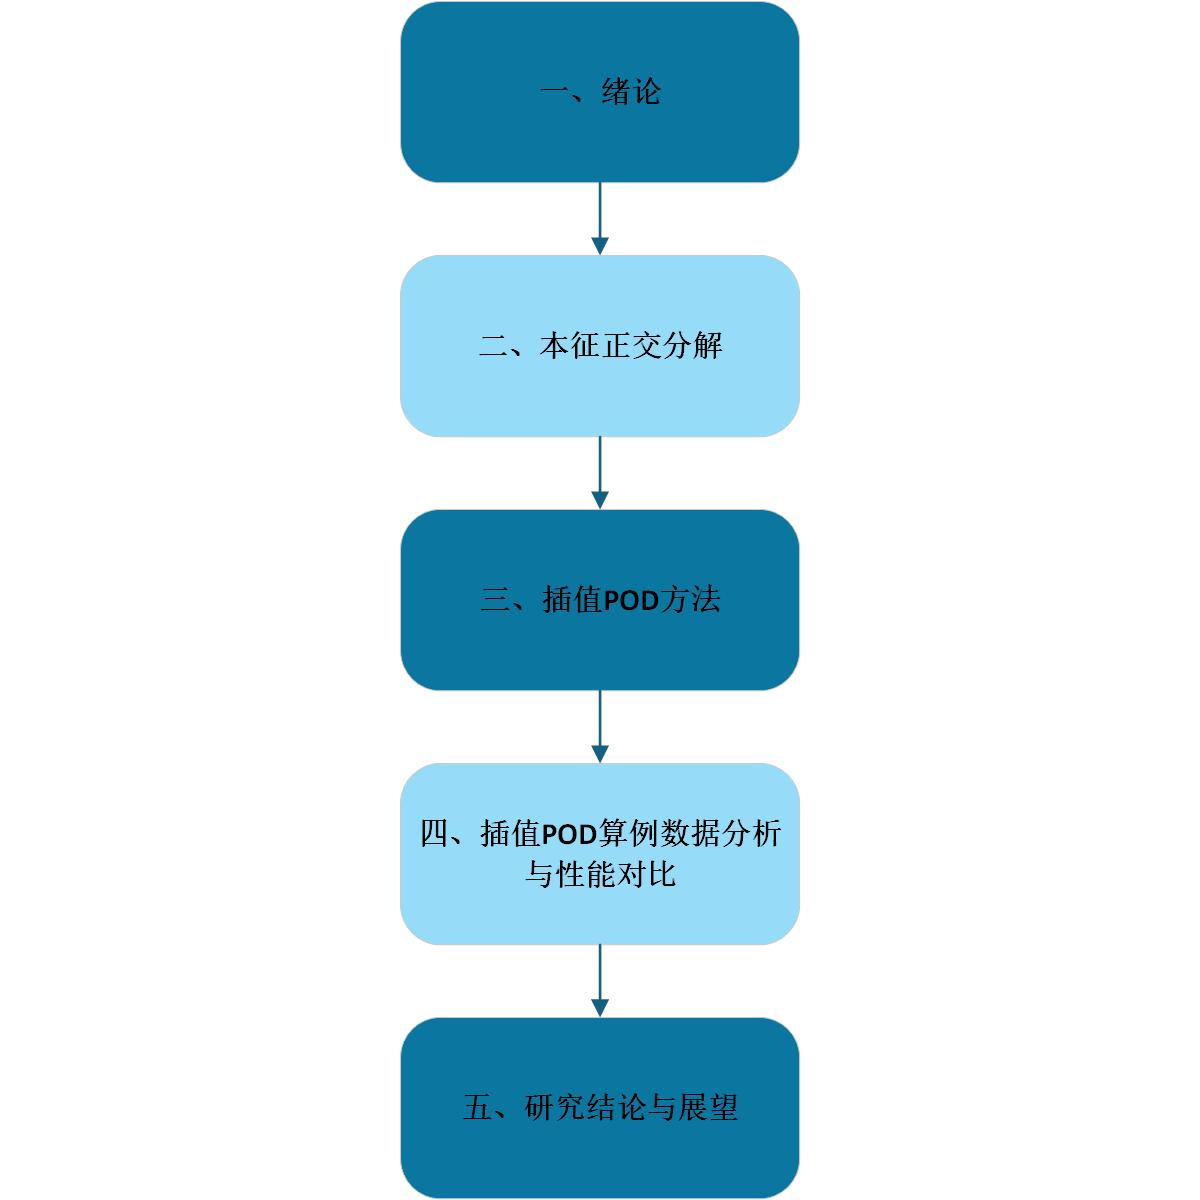
\includegraphics[width=1.0\linewidth]{论文结构图.jpg}
    \caption{论文组织结构图}
    \label{fig:enter-label}
\end{figure}
本章通过分析工程需求、梳理研究现状及明确技术路径,为后续 POD 理论推导、翼型模型建立及重构方法实现奠定基础。
\newclearpage
                \chapter{基本理论方法}
\label{cha:sysu-thesis-contents-format-requirement}

\section{本征正交分解方法原理}

给定 $n$ 维空间中的 $m$ 个快照向量 $\mathbf{s}_i \in \mathbb{R}^n$ 构成数据矩阵 $S = [\mathbf{s}_1\ \mathbf{s}_2\ \cdots\ \mathbf{s}_m]$,POD 方法通过求解以下优化问题构建最优正交基:

\begin{equation}
    \max_{\{\phi_j\}} \sum_{j=1}^k \mathbb{E}[(\mathbf{s},\phi_j)^2] \quad \text{s.t.} \quad \phi_i^T\phi_j = \delta_{ij}
    \label{eq:pod_optimization}
\end{equation}

该优化问题的物理意义在于寻找一组正交基,使得这些基向量能够捕捉数据中最大的方差。换句话说,POD 方法试图用尽可能少的基向量来描述数据的主要特征,从而实现降维。

引入拉格朗日乘子 $\lambda_j$ 处理正交约束:

\begin{equation}
    \mathcal{L} = \sum_{j=1}^k \phi_j^T S S^T \phi_j - \sum_{j=1}^k \lambda_j (\phi_j^T\phi_j - 1)
    \label{eq:lagrangian}
\end{equation}

对 $\phi_j$ 求导并令导数为零,得到特征方程:

\begin{equation}
    \frac{\partial \mathcal{L}}{\partial \phi_j} = 2S S^T \phi_j - 2\lambda_j \phi_j = 0 \Rightarrow S S^T \phi_j = \lambda_j \phi_j
    \label{eq:eigen_equation}
\end{equation}

这表明 POD 基向量实际上是数据协方差矩阵的特征向量,对应的特征值衡量了每个基向量所包含的信息量。

\subsection{经典 POD 方法}
经典 POD (Classical POD) 是由 Lumley 在 1967 年提出的,它是最直接的 POD 实现方式。
\begin{equation}
R \phi_j = \lambda_j \phi_j, \quad \phi_j \in \mathbb{R}^n, \lambda_1 \geq \lambda_2 \geq \cdots \geq \lambda_n \geq 0
\end{equation}

其中,$R$ 代表协方差矩阵:

\begin{equation}
R = \frac{1}{m} \sum_{i=1}^m s_i s_i^T = S S^T \in \mathbb{R}^{n \times n}
\end{equation}

公式 (2.4) 所求得的特征向量 $\phi_j$ 就是 POD 基,它们是单位正交的,这也意味着:
\begin{equation}
\phi_j^T \phi_k = 
\begin{cases} 
0, & j \neq k \\
1, & j = k 
\end{cases}
\end{equation}

特征值 $\lambda_j$ 越大,就说明其对应的 POD 基 $\phi_j$ 包含这个矩阵 $S$ 的信息越多。将 POD 基按照其对应的特征值大小排序后,就可以得到有序的一组单位正交 POD 基。通常情况下,往往只保留前 k 个基来表达原始数据,在 $k$ 的选择上通常使用能量阈值法,设阈值为 $\epsilon_\sigma$,当满足式 (2.7) 时,确定 k 值,$\epsilon_\sigma$ 由设计者决定:

\begin{equation}
\frac{\sum_{j=1}^k \lambda_j}{\sum_{j=1}^n \lambda_j} \geq \epsilon_\sigma
\end{equation}

确定使用数量 k 后,用 POD 基来表达数据向量空间中的任意向量可得:

\begin{equation}
s \approx \sum_{j=1}^k \beta_j \phi_j
\end{equation}

其中,系数 $\beta_j$ 可以通过式 (2.9) 求出:

\begin{equation}
\beta_j = s^T \phi_j
\end{equation}
\subsection{快照 POD }
快照 POD 方法 (Snapshot POD) 是 Sirovich 等人提出的,也是目前气体设计领域最常用的 POD 方法。经典 POD 求解的实际上是 $R = S S^T$ 的特征值分解问题,$R$ 的大小是 $n \times n$。当 $n$ 的数值较大时,特征值分解所需消耗的时间将会显著增加。因此,当出现 $m \ll n$ 的时候就可以采用快照 POD 方法,快照 POD 方法求解的问题是:
\begin{equation}
S^T S \psi_j = \sigma_j \psi_j, \quad \psi_j \in \mathbb{R}^m, \sigma_1 \geq \sigma_2 \geq \cdots \geq \sigma_m \geq 0
\end{equation}

其中,$S^T S$ 是一个大小为 $m \times m$ 的协方差矩阵。在进行特征值分解时,$S^T S$ 和 $S S^T$ 的特征值都是相同的。另外,式 (2.10) 是从数学上对快照 POD 的描述,因此省去了 $\frac{1}{m}$ 的系数,

求出来的特征向量 $\psi_j$ 可以通过式 (2.11) 转换为 POD 基 $\phi_j$:

\begin{equation}\phi_{j}=S\psi_{j}\frac{1}{\sqrt{\lambda_{j}}}\in\mathbb{R}^{n},\quad j=1,2,\cdots,m\end{equation}

用矩阵形式描述为:

\begin{equation}
\Phi = S \Psi \Sigma^{-1/2}
\end{equation}

其中,$\Phi = [\phi_1 \phi_2 \cdots \phi_m] \in \mathbb{R}^{n \times m}$,$\Psi = [\psi_1 \psi_2 \cdots \psi_m] \in \mathbb{R}^{m \times m}$。
\subsection{SVD-POD}
对于数据矩阵 $S \in \mathbb{R}^{n \times m}$,实际上可以直接进行 SVD 分解:

\begin{equation}
S = \Phi \Sigma \Psi^T
\end{equation}

其中,$U$ 的列向量称为左奇异向量,$\Sigma$ 是奇异值矩阵,$V$ 的列向量称为右奇异向量。经济型 SVD 分解仅保留与数据秩相关的部分,避免计算冗余的零奇异值。

左奇异向量矩阵 $U$ 即为 POD 基:

\begin{equation}
    \sigma_j^2 = m\lambda_j, \quad \phi_j = U(:,j)
    \label{eq:svd_relation}
\end{equation}

这表明 SVD 分解中的左奇异向量与 POD 基在数学上是等价的,而奇异值的平方与 POD 特征值成正比。

通过矩阵分解理论可证:

\begin{equation}
    \mathbf{R} = \frac{1}{m}U\Sigma^2 U^T \Rightarrow U \equiv \Phi
    \label{eq:equivalence_proof}
\end{equation}

这表明经典 POD 方法中的协方差矩阵分解与 SVD 分解中的左奇异向量矩阵是相同的,从而证明了两种方法的等价性。


\section{矩阵特征值求解方法}

在科学技术的应用领域中,许多问题都可以归结为求解一个特征系统。如动力学系统和机构振动中的振动问题,求系统的频率与振型等等。矩阵特征值问题的数学表述如下:

设 \(\mathbf{A}\) 为 \(n\) 阶实矩阵,若有 \(n\) 维非零向量 \(\mathbf{x}\),有数 \(\lambda\) 使\begin{equation}
\mathbf{A}\mathbf{x} = \lambda \mathbf{x} 
\end{equation}

则称 \(\lambda\) 为 \(\mathbf{A}\) 的特征值,\(\mathbf{x}\) 为相应于 \(\lambda\) 的特征向量。线性代数理论中式通过求解特征多项式 \(\det(\mathbf{A} - \lambda \mathbf{I}) = 0\) 求得特征值,进而求得特征向量。当矩阵的阶数较高时,这种方法极为困难,所以常用数值方法来求解特征问题。常用的数值方法可以分为迭代法和变换法两种。变换法适用于中小型矩阵,常用的有适用于实对称矩阵的 Jacobi 方法,奇异值分解方法等等。

POD 方法中自相关矩阵均是实对称矩阵,而且一般阶数都不会很高,因此选用变换法中的 Jacobi 方法和奇异值分解求解矩阵的特征值与特征向量。在此对这两种方法做简单介绍。

\subsection{Jacobi 变换方法}

Jacobi 变换方法是求实对称矩阵全部特征值及对应特征向量的一种变换方法。其基本思想是把实对称矩阵经一系列正交相似变换约化为一个近似对角阵,即:

\begin{equation}
\left\{
\begin{aligned}
\mathbf{A}_0 &= \mathbf{A} \\
\mathbf{A}_{k+1} &= \mathbf{R}_{k+1}^T \mathbf{A}_k \mathbf{R}_{k+1} \quad k = 0, 1, 2, \ldots
\end{aligned}
\right. 
\end{equation}

最终对角阵的对角元就是该矩阵的近似特征值,由各个正交变换阵的乘积可得对应的特征向量。

一般选取 Givens 旋转矩阵做相似变换阵。该矩阵定义如下:


\begin{equation}
\mathbf{R}(p,q,\theta)=\begin{bmatrix} 1 & & & & & & & \\ & \ddots & & & & & & \\ & & 1 & & & & & \\ & & & \cos\theta & \cdots & \sin\theta & & \\ & & & \vdots & \vdots & \vdots & & \\ & & & -\sin\theta & \cdots & \cos\theta & & \\ & & & & & & \ddots & \\ & & & & & & & 1 \\\end{bmatrix} 
\end{equation}
它是在单位阵 \(\mathbf{I}\) 的 \(p\) 行、\(q\) 行和 \(p\) 列、\(q\) 列的四个交叉位置上分别置 \(\cos\theta\),\(\sin\theta\),\(-\sin\theta\) 和 \(\cos\theta\) 而成的。容易验证旋转矩阵是正交矩阵,即 \(\mathbf{R}^T(p, q, \theta) = \mathbf{R}^{-1}(p, q, \theta)\),所以用它做相似变换阵时十分方便。

综上,Jacobi 变换法的计算步骤为:

\begin{enumerate}
    \item 令 \(\mathbf{H}_{k+1}^T = \mathbf{I}\),\(k = 0\),确定 \(\varepsilon\);
    \item 确定 \(p\),\(q\)(\(p < q\)),使 \(|a_{pq}^{(k)}| = \max_{i < j} |a_{ij}^{(k)}|\);
    \item 若 \(|a_{pq}^{(k)}| < \varepsilon\),则停止计算,对角矩阵的元素即为特征值,\(\mathbf{H}_k\) 的列向量即为特征向量;
    \item 计算 \(\cos\theta\),\(\sin\theta\),获得 Givens 变换阵 \(\mathbf{R}_{pq}\):
    
    通常将 \(\theta\) 限制在 \(\left[ -\frac{\pi}{4}, \frac{\pi}{4} \right]\),具体求法如下:
    
    当 \(a_{pp}^{(k)} = a_{qq}^{(k)}\),取 \(\cos\theta = \frac{\sqrt{2}}{2}\),\(\sin\theta = \text{sign}(a_{pq}^{(k)}) \cos\theta\);
    
    当 \(a_{pp}^{(k)} \neq a_{qq}^{(k)}\),取 \(\cos\theta = \frac{1}{\sqrt{1 + t^2}}\),\(\sin\theta = t \cos\theta\),其中 \(t = \tan\theta = \frac{\text{sign}(d)}{|d| + \sqrt{d^2 + 1}}\),\(d = \frac{a_{pp}^{(k)} - a_{qq}^{(k)}}{2 a_{pq}^{(k)}}\)。\(a\) 是迭代中所求矩阵的元素,\(k\) 表示迭代的步数。
    \item 计算 \(\mathbf{H}_{k+1}^T = \mathbf{H}_k^T \mathbf{R}_{pq}\),\(\mathbf{A}_{k+1} = \mathbf{R}_{pq}^T \mathbf{A}_k \mathbf{R}_{pq}\),返回(2)。
\end{enumerate}

\subsection{奇异值分解方法}

对于实矩阵 \(\mathbf{A} \in \mathbb{R}^{m \times n}\),\(\mathbf{A}^T \mathbf{A}\) 的特征值为 \(\lambda_1 \geq \lambda_2 \geq \cdots \geq \lambda_n \geq 0\),则称 \(\sigma_i = \sqrt{\lambda_i}\)(\(i = 1, 2, \ldots, n\))为 \(\mathbf{A}\) 的奇异值。对于上述矩阵 \(\mathbf{A}\),存在 \(m\) 阶正交矩阵 \(\mathbf{U}\) 和 \(n\) 阶正交矩阵 \(\mathbf{V}\),使得:

\begin{equation}
\mathbf{U}^T \mathbf{A} \mathbf{V} = \begin{pmatrix} \mathbf{\Sigma} & \mathbf{0} \\ \mathbf{0} & \mathbf{0} \end{pmatrix} 
\end{equation}

其中 \(\mathbf{\Sigma} = \text{diag}(\sigma_1, \sigma_2, \ldots, \sigma_r)\),将上式改写为:

\begin{equation}
\mathbf{A} = \mathbf{V} \begin{pmatrix} \mathbf{\Sigma} & \mathbf{0} \\ \mathbf{0} & \mathbf{0} \end{pmatrix} \mathbf{U}^T 
\end{equation}

称之为 \(\mathbf{A}\) 的奇异值分解。

设 \(\mathbf{A} \in \mathbb{R}^{n \times n}\) 为实对称矩阵,其特征值为 \(\lambda_i(\mathbf{A})\)(\(i = 1, 2, \ldots, n\)),因为对实对称矩阵有 \(\mathbf{A} = \mathbf{A}^T\),所以:

\begin{equation}
\lambda_i(\mathbf{A}^T \mathbf{A}) = \lambda_i(\mathbf{A}^2) = \left[ \lambda_i(\mathbf{A}) \right]^2 \quad (i = 1, 2, \ldots, n) 
\end{equation}
A 的奇异值 \(\sigma_i = \sqrt{\lambda_i(\mathbf{A}^T \mathbf{A})} = \lambda_i(\mathbf{A})\)(\(i = 1, 2, \ldots, n\))。至此,我们可以知道,对于实对称矩阵,它的奇异值和它的特征值是相同的。只要得到 A 的奇异值分解:

\begin{equation}
\mathbf{A} = \mathbf{V}^T \mathbf{\Sigma} \mathbf{U} 
\end{equation}

则 A 的特征值为 \(\mathbf{\Sigma}\) 中的对角元素,对应特征向量为 \(\mathbf{V}^T\) 的列向量。

一般实矩阵的奇异值分解要首先使用 Householder 变换把矩阵化为双对角线矩阵,再用 QR 算法迭代求解奇异值,上述两种方法较为常见,本文不再赘述。
\section{气动分析方法}
使用 POD 方法的前提是有准确的流场求解方法,以提供合理的采样解。本文所作的工作都是针对要型流场进行的,其中进行方法验证时一般都使用的欧拉方程求解器,以缩短验算周期。在与优化相关的问题中使用的是 NS 方程求解器。鉴于二维定常 NS 方程的数值求解技术已臻成熟,且本文重点不在于此,故只对二维定常 NS 方程的数值求解方法做简单介绍。

从欧拉运动描述的观点出发,在任何有限控制体内的流动,质量、动量、能量所发生的暂时性变化,必须通过流入流出控制体的通量和控制体内部的当地变化来平衡。对于大多空气动力学中的应用来说,流动内部不存在热源或质量源,通常情况下,体积力(或彻体力)的影响,例如重力是可以忽略不计的。于是,控制方程式可以写成如下积分形式:

\begin{equation}
\frac{\partial}{\partial t} \iiint_V \mathbf{W} \, dV + \iint_S \mathbf{F} \cdot \mathbf{n} \, dS = 0 
\end{equation}

式中,\(V\) 是一个有封闭边界 \(S\) 的任意控制体,\(\mathbf{n}\) 为边界的法向量;指向朝外,状态变量 \(\mathbf{W}\) 的表达式为:

\begin{equation}
\mathbf{W} = (\rho, \rho u, \rho v, \rho E)^T 
\end{equation}

其中 \(\rho\) 为密度,\(u, v\) 是两个个笛卡尔速度分量,\(E\) 是单位质量流体的总能量,表达式为:

\begin{equation}
E = e + \frac{1}{2}(u^2 + v^2) 
\end{equation}

其中 \(e\) 是内能,方程(4-1)中的矢通量 \(\mathbf{F}\) 可分解成对流项(无粘部分)\(\mathbf{F}_c\) 和耗散项(粘性和热传递部分)\(\mathbf{F}_d\),即:
\begin{equation}
\mathbf{F} = \mathbf{F}_c + \mathbf{F}_d 
\end{equation}

对流通量表达式为:

\begin{equation}
\mathbf{F}_c = 
\begin{bmatrix}
\rho u i & \rho v j \\
(\rho u^2 + p) i & \rho u v j \\
\rho v u i & (\rho v^2 + p) j \\
(\rho E u + \rho u) i & (\rho E v + \rho v) j
\end{bmatrix} 
\end{equation}

其中,\(i, j\) 是直角坐标系的单位向量,通量的粘性应力项和热扩散的状态方程为:

\begin{equation}
\mathbf{F}_d = 
\begin{bmatrix}
0 & 0 \\
\tau_{x,i} & \tau_{x,j} \\
\tau_{y,i} & \tau_{y,j} \\
(u \tau_x + v \tau_y - q_x) i & (u \tau_x + v \tau_y - q_y) j
\end{bmatrix} 
\end{equation}

各个方向的剪应力及热通量可被定义为:
\begin{align}
\tau_{x,i} &= 2(\mu + \mu_t) \frac{\partial u}{\partial x} - \frac{2}{3} (\mu + \mu_t) \left( \frac{\partial u}{\partial x} + \frac{\partial v}{\partial y} \right) \\
\tau_{y,i} &= 2(\mu + \mu_t) \frac{\partial v}{\partial y} - \frac{2}{3} (\mu + \mu_t) \left( \frac{\partial u}{\partial x} + \frac{\partial v}{\partial y} \right) \\
\tau_{x,j} &= \tau_{x,i} = (\mu + \mu_t) \left( \frac{\partial u}{\partial y} + \frac{\partial v}{\partial x} \right)  \\
q_x &= -(k + k_t) \frac{\partial T}{\partial x} \\
q_y &= -(k + k_t) \frac{\partial T}{\partial y}
\end{align}

其中 \(\mu\) 表示层流粘性系数,\(\mu_t\) 表示湍流粘性系数,\(k\) 表示层流导热系数,\(k_t\) 表示湍流导热系数,\(T\) 表示温度。

总焓可以表示为:

\begin{equation}
H = h + \frac{1}{2}(u^2 + v^2)
\end{equation}

完全气体的定义和关系由下面的状态方程给出:

\begin{equation}
e = c_v T, \quad h = c_p T, \quad R = c_p - c_v, \quad \gamma = \frac{c_p}{c_v} 
\end{equation}

理想气体状态方程如下:

\begin{equation}
\frac{p}{\rho} = RT 
\end{equation}
压力和总焓可被表示为:

\begin{equation}
H = E + \frac{p}{\rho} 
\end{equation}

即
\begin{equation}
p = (\gamma - 1) \rho \left[ E - \frac{1}{2}(u^2 + v^2) \right] 
\end{equation}

其中,\(c_p\) 和 \(c_v\) 分别表示恒压和恒容比热,\(\gamma\) 是比热比,\(R\) 是气体常数,温度 \(T\) 由此给出:
\begin{equation}
T = \frac{\gamma}{c_v (\gamma - 1) \rho} p 
\end{equation}

由 Sutherland's 方程得到层流粘性系数公式:

\begin{equation}
\frac{\mu}{\mu_\infty} = \left( \frac{T}{T_\infty} \right)^{\frac{3}{2}} \frac{T_\infty + 110.3}{T + 110.3} 
\end{equation}

最终,完全气体声速为:

\begin{equation}
a = \sqrt{\frac{\gamma p}{\rho}} 
\end{equation}

马赫数为:

\begin{equation}
M = \frac{\sqrt{u^2 + v^2 + w^2}}{a}
\end{equation}

该方程在数值求解时:空间离散使用格心格式的有限体积法,时间推进采用显式 5 步龙格库塔迭代方法。使用 \(k-\omega\) 端流模型。物面边界使用绝热的无滑移边界条件,远场边界使用无反射边界条件。加入人工粘性项以保证算法的稳定及抑制激波附近的震荡。使用隐式残值光顺和多重网格的加速收敛技术。

\section{单变量三次样条插值法}
\subsection{数学描述}
考虑定义在区间$[a,b]$上的三次样条插值问题。给定节点$\{x_0,x_1,...,x_n\}$及其对应函数值$\{f(x_i)\}$,要求构造分段三次多项式函数$S(x)$满足:

\begin{enumerate}
    \item 在子区间$[x_i, x_{i+1}]$上的局部表达式为:
    \begin{equation}
        S_i(x) = a_i + b_i(x-x_i) + c_i(x-x_i)^2 + d_i(x-x_i)^3
    \end{equation}
    \item 整体满足$C^2$连续性:
    \begin{align}
        \lim_{x\to x_i^+} S^{(k)}(x) &= \lim_{x\to x_i^-} S^{(k)}(x), \quad k=0,1,2
    \end{align}
    \item 自然边界条件:
    \begin{equation}
        S''(x_0) = S''(x_n) = 0
    \end{equation}
\end{enumerate}
\subsection{系数求解}
令$M_i = S''(x_i)$,根据三次多项式的二阶导数特性,可得递推关系:
\begin{equation}
    \frac{h_{i-1}}{6}M_{i-1} + \frac{h_{i-1}+h_i}{3}M_i + \frac{h_i}{6}M_{i+1} = \frac{f(x_{i+1})-f(x_i)}{h_i} - \frac{f(x_i)-f(x_{i-1})}{h_{i-1}}
\end{equation}
其中$h_i = x_{i+1}-x_i$。该方程组可表示为三对角矩阵形式:
\begin{equation}
    \begin{pmatrix}
        2 & \lambda_1 & 0 & \cdots & 0 \\
        \mu_2 & 2 & \lambda_2 & \cdots & 0 \\
        \vdots & \ddots & \ddots & \ddots & \vdots \\
        0 & \cdots & \mu_{n-1} & 2 & \lambda_{n-1} \\
        0 & \cdots & 0 & \mu_n & 2
    \end{pmatrix}
    \begin{pmatrix}
        M_1 \\ M_2 \\ \vdots \\ M_{n-1} \\ M_n
    \end{pmatrix}
    = \mathbf{b}
\end{equation}
其中$\mu_i = h_{i-1}/(h_{i-1}+h_i)$,$\lambda_i = 1-\mu_i$,右端项$\mathbf{b}$由差商计算。通过Thomas算法可高效求解该方程组。

对于形如$A\mathbf{M} = \mathbf{b}$的三对角方程组:
\[
\begin{pmatrix}
    b_1 & c_1 & 0 & \cdots & 0 \\
    a_2 & b_2 & c_2 & \cdots & 0 \\
    0 & \ddots & \ddots & \ddots & \vdots \\
    \vdots & & a_{n-1} & b_{n-1} & c_{n-1} \\
    0 & \cdots & 0 & a_n & b_n
\end{pmatrix}
\begin{pmatrix}
    M_1 \\ M_2 \\ \vdots \\ M_{n-1} \\ M_n
\end{pmatrix}
= 
\begin{pmatrix}
    d_1 \\ d_2 \\ \vdots \\ d_{n-1} \\ d_n
\end{pmatrix}
\]
采用追赶法(Thomas算法)进行高效求解,其计算步骤如下:

\begin{enumerate}
    \item {向前消元}:计算修正系数
    \begin{align}
        c'_1 &= \frac{c_1}{b_1} \\
        d'_1 &= \frac{d_1}{b_1} \\
        c'_i &= \frac{c_i}{b_i - a_i c'_{i-1}}, \quad i=2,...,n-1 \\
        d'_i &= \frac{d_i - a_i d'_{i-1}}{b_i - a_i c'_{i-1}}, \quad i=2,...,n
    \end{align}

    \item{向后回代}:求解节点二阶导数
    \begin{align}
        M_n &= d'_n \\
        M_i &= d'_i - c'_i M_{i+1}, \quad i=n-1,n-2,...,1
    \end{align}
\end{enumerate}

在三次样条插值的具体场景中:
\begin{itemize}
    \item 主对角线元素:$b_i = \frac{h_{i-1} + h_i}{3}$
    \item 次对角线元素:$a_i = \frac{h_{i-1}}{6}$
    \item 超对角线元素:$c_i = \frac{h_i}{6}$
    \item 右端项:$d_i = \frac{f(x_{i+1}) - f(x_i)}{h_i} - \frac{f(x_i) - f(x_{i-1})}{h_{i-1}}$
\end{itemize}

该算法的时间复杂度为$O(n)$,显著优于高斯消元法的$O(n^3)$,特别适用于大规模网格计算\cite{deboor1978}。
\section{双变量三次样条插值法}
\subsection{基本定义与条件}
设矩形区域$U = [a,b] \times [c,d]$被划分为$m \times n$个网格,双变量三次样条插值函数$S(x,y)$需满足:
\begin{enumerate}
    \item {局部双三次性}:在子区域$[x_i,x_{i+1}] \times [y_j,y_{j+1}]$内,$S(x,y)$为双三次多项式
    \item{全局光滑性}:$S(x,y) \in C^{2,2}(U)$,即二阶混合偏导数连续
    \item {插值条件}:$S(x_i,y_j) = z_{ij},\ \forall i=0,1,...,m; j=0,1,...,n$
\end{enumerate}
\subsection{张量积构造方法}
基于一维三次样条的张量积扩展,构造方法可分两步实现:

\begin{enumerate}
    \item 固定$y = y_j$,构造$x$方向三次样条:
    \begin{equation}
        S_j(x) = \sum_{k=0}^3 a_{jk}(x-x_i)^k,\quad x \in [x_i,x_{i+1}]
    \end{equation}
    系数$a_{jk}$通过以下条件确定:
    \begin{align}
        S_j(x_i) &= z_{ij} \\
        S_j'(x_i^+) &= S_j'(x_i^-) \\
        S_j''(x_i^+) &= S_j''(x_i^-)
    \end{align}
    
    \item 对每个$x_i$构造$y$方向样条:
    \begin{equation}
        S_i(y) = \sum_{l=0}^3 b_{il}(y-y_j)^l,\quad y \in [y_j,y_{j+1}]
    \end{equation}
    最终的双变量样条表示为:
    \begin{equation}
        S(x,y) = \sum_{i=1}^m \sum_{j=1}^n \alpha_{ij} B_i^{(3)}(x) B_j^{(3)}(y)
    \end{equation}
    其中$B^{(3)}$为三次B样条基函数\cite{deboor1978}。
\end{enumerate}
\subsection{连续性条件}
为保证$C^{2,2}$连续性,需满足以下条件:
\begin{enumerate}
    \item 函数值连续:$\lim_{\epsilon \to 0} S(x_i \pm \epsilon, y_j) = z_{ij}$
    \item 一阶偏导连续:
    \begin{equation}
        \frac{\partial S}{\partial x}\bigg|_{(x_i^+,y_j)} = \frac{\partial S}{\partial x}\bigg|_{(x_i^-,y_j)}
    \end{equation}
    \item 二阶混合偏导连续:
    \begin{equation}
        \frac{\partial^2 S}{\partial x \partial y}\bigg|_{(x_i^+,y_j^+)} = \frac{\partial^2 S}{\partial x \partial y}\bigg|_{(x_i^-,y_j^-)}
    \end{equation}
\end{enumerate}
\subsection{算法实现}
核心算法流程如下:
\begin{enumerate}
    \item 输入:网格节点$\{(x_i,y_j)\}_{i,j=0}^{m,n}$,对应函数值$\{z_{ij}\}$
    \item 对每个$y_j$,求解三对角方程组:
    \begin{equation}
        \begin{bmatrix}
        2 & 1 & & \\
        1 & 4 & 1 & \\
        & \ddots & \ddots & \ddots \\
        & & 1 & 2
        \end{bmatrix}
        \begin{bmatrix}
        M_{1j} \\ M_{2j} \\ \vdots \\ M_{mj}
        \end{bmatrix}
        = 6
        \begin{bmatrix}
        \frac{z_{1j}-z_{0j}}{h_1} - \frac{z_{0j}-z_{-1j}}{h_0} \\
        \vdots \\
        \frac{z_{mj}-z_{m-1j}}{h_m} - \frac{z_{m-1j}-z_{m-2j}}{h_{m-1}}
        \end{bmatrix}
    \end{equation}
    其中$M_{ij}$为二阶导数在节点处的值
    \item 类似地构造$y$方向样条
    \item 合成双变量样条表达式
\end{enumerate}


% \subsection{正文}

% 正文是毕业论文的主体和核心部分,不同学科专业和不同的选题可以有不同的写作方式。正文一般包括以下几个方面:

% \begin{enumerate}
%     \item \textbf{绪论} \\
%           绪论应包括毕业论文选题的背景、目的和意义;对国内外研究现状和相关领域中已有的研究成果的简要评述;介绍本项研究工作研究设想、研究方法或实验设计、理论依据或实验基础;涉及范围和预期结果等。要求言简意赅,注意不要与摘要雷同或成为摘要的注解。
%     \item \textbf{主体} \\
%           论文主体是毕业论文的主要部分,必须言之成理,论据可靠,严格遵循本学科国际通行的学术规范。在写作上要注意结构合理、层次分明、重点突出,章节标题、公式图表符号必须规范统一。论文主体的内容根据不同学科有不同的特点,一般应包括以下几个方面:
%           \begin{enumerate}
%               \item 毕业论文总体方案或选题的论证;
%               \item 毕业论文各部分的设计实现,包括实验数据的获取、数据可行性及有效性的处理与分析、各部分的设计计算等;
%               \item 对研究内容及成果的客观阐述,包括理论依据、创新见解、创造性成果及其改进与实际应用价值等;
%               \item 论文主体的所有数据必须真实可靠,凡引用他人观点、方案、资料、数据等,无论曾否发表,无论来源于纸质或电子版材料,均应详加注释。自然科学论文应推理正确、结论清晰;人文和社会学科的论文应把握论点正确、论证充分、论据可靠,恰当运用系统分析和比较研究的方法进行模型或方案设计,注重实证研究和案例分析,根据分析结果提出建议和改进措施等。
%           \end{enumerate}
%     \item \textbf{结论} \\
%           结论是毕业论文的总结,是整篇论文的归宿,应精炼、准确、完整。结论应着重阐述自己的创造性成果及其在本研究领域中的意义和作用,还可进一步提出需要讨论的问题和建议。
% \end{enumerate}

% \subsection{参考文献}

% 参考文献是毕业论文不可缺少的组成部分,它反映毕业论文的取材来源、材料的广博和可靠程度,也是作者对他人知识成果的承认和尊重。凡有引用他人的著作、论文等,均应列于参考文献中。

% \subsection{相关的科研成果目录}

% 本科期间发表的与毕业论文相关的论文或被鉴定的技术成果、发明专利等,应在成果目录中列出。此项不是必需项,空缺时可以省略。

% \subsection{附录}

% 对于一些不宜放在正文中的重要支撑材料,可编入毕业论文的附录中,包括某些重要的原始数据、详细数学推导、程序全文及其说明、复杂的图表、设计图纸等一系列需要补充提供的说明材料。如果毕业论文中引用的实例、数据资料,实验结果等符号较多时,为了节约篇幅,便于读者查阅,可以编写一个符号说明,注明符号代表的意义。附录的篇幅不宜太多,一般不超过正文。此项不是必需项,空缺时可以省略。

% \subsection{致谢}

% 致谢应以简短的文字对课题研究与论文撰写过程中曾直接给予帮助的人员(例如指导教师、答疑教师及其他人员)表达自己的谢意,这不仅是一种礼貌,也是对他人劳动的尊重,是治学者应当遵循的学术规范。内容限一页。


% \section{毕业论文的撰写格式要求}


% \subsection{文字和字数}


% 除外国语言文学类专业外,其他专业的毕业论文须采用简化汉语文字撰写。论文正文部分一般不少于8000 字,各专业可根据需要确定具体的字数要求,并报教务部备案。

% \subsection{字体和字号}

% 标题一般用黑体,内容一般用宋体,数字和英文字母一般用Times New Roman,具体如\autoref{tab:font-spec}。

% \begin{table}[]
%     \caption{字体使用规范}
%     \begin{tabular}{|c|c|}
%         \hline
%         论文题目               & 黑体二号居中                                  \\ \hline
%         中文摘要标题           & 黑体三号居中                                  \\ \hline
%         中文摘要内容           & 宋体小四号                                    \\ \hline
%         中文关键词             & 宋体小四号(标题``关键词''加粗)              \\ \hline
%         英文摘要标题           & Times New Roman加粗三号全部大写               \\ \hline
%         英文摘要内容           & Times New Roman小四号                         \\ \hline
%         英文关键词             & Times New Roman小四号(标题``Keywords''加粗) \\ \hline
%         目录标题               & 黑体三号居中                                  \\ \hline
%         目录内容               & 宋体小四号                                    \\ \hline
%         正文各章标题           & 黑体三号居中                                  \\ \hline
%         正文各节一级标题       & 黑体四号左对齐                                \\ \hline
%         正文各节二级及以下标题 & 宋体小四号加粗左对齐空两格                    \\ \hline
%         正文内容               & 宋体小四号                                    \\ \hline
%         参考文献标题           & 黑体三号居中                                  \\ \hline
%         参考文献内容           & 宋体五号                                      \\ \hline
%         致谢、附录标题         & 黑体三号居中                                  \\ \hline
%         致谢、附录内容         & 宋体小四号                                    \\ \hline
%         页眉与页脚             & 宋体五号居中                                  \\ \hline
%         图题、表题             & 宋体五号                                      \\ \hline
%         脚注、尾注             & 宋体小五号                                    \\ \hline
%     \end{tabular}
%     \label{tab:font-spec}
% \end{table}


% 字体样例可见如下(以居中形式展现): \\



% \begin{center}
%     {\heiti\zihao{2}黑体二号居中} \\

%     {\heiti\zihao{3}黑体三号居中} \\

%     {\heiti\zihao{4}黑体四号居中} \\

%     {\songti\zihao{4}宋体四号居中} \\

%     {\songti\zihao{-4}宋体小四号居中} \\

%     {\songti\zihao{5}宋体五号居中} \\

%     {\songti\zihao{-5}宋体小五号居中} \\

%     {\zihao{3} Times New Roman : Three} 三号居中 \\

%     {\zihao{-4} Times New Roman : Small Four} 小四号居中 \\

% \end{center}


% \subsection{页面设置}

% 纸张大小:A4。

% 页边距:上边距25 mm,下边距20 mm,左右边距均为30 mm。

% 行距:1.5倍行距,章和节标题段前段后各空0.5行。

% \subsection{页码}

% 页面底端居中,从摘要开始至绪论之前以大写罗马数字(
% \uppercase\expandafter{\romannumeral1} ,
% \uppercase\expandafter{\romannumeral2} ,
% \uppercase\expandafter{\romannumeral3} ,
% …)单独编连续码,绪论开始至论文结尾,以阿拉伯数字(1,2,3…)编连续码。

% \subsection{关键词}


% 摘要正文下方另起一行顶格打印``关键词''款项,后加冒号,多个关键词以逗号分隔。

% \subsection{目录}

% 目录应另起一页,包括论文中的各级标题,按照``一……''、``(一)……''或``1……''、``1.1……''格式编写。

% \subsection{各级标题}

% 正文各部分的标题应简明扼要,不使用标点符号。论文内文各大部分的标题用``一、二……(或1、2……)'',次级标题为``(一)、(二)……(或1.1、2.1……)'',三级标题用``1、2……(或1.1.1、2.1.1……)'',四级标题用``(1)、(2)……(或1.1.1.1、2.1.1.1……)'',不再使用五级以下标题。两类标题不要混编。

% \subsection{名词术语}

% \begin{enumerate}
%     \item 科学技术名词术语尽量采用全国自然科学名词审定委员会公布的规范词或国家标准、部标准中规定的名称,尚未统一规定或叫法有争议的名词术语,可采用惯用的名称。
%     \item 特定含义的名词术语或新名词、以及使用外文缩写代替某一名词术语时,首次出现时应在括号内注明其含义,如:经济合作与发展组织(Organisation for Economic Co-operation and Development, OECD)。
%     \item 外国人名一般采用英文原名,可不译成中文,英文人名按姓前名后的原则书写,如:CRAY P,不可将外国人姓名中的名部分漏写,例如:不能只写CRAY, 应写成CRAY P。一般很熟知的外国人名(如牛顿、爱因斯坦、达尔文、马克思等)可按通常标准译法写译名。
% \end{enumerate}

% \subsection{物理量名称、符号与计量单位}

% \begin{enumerate}
%     \item 论文中某一物理量的名称和符号应统一,应采用国务院发布的《中华人民共和国法定计量单位》、国际公认或各行业领域惯用的计量单位。单位名称和符号的书写方式,应采用国际通用符号。
%     \item 在不涉及具体数据表达时允许使用中文计量单位如``千克''。
%     \item 表达时刻应采用中文计量单位,如``下午3点10分'',不能写成``3h10min'',在表格中可以用``3:10PM''表示。
%     \item 物理量符号、物理量常量、变量符号用斜体,计量单位符号均用正体。
% \end{enumerate}

% \subsection{数字}

% \begin{enumerate}
%     \item 无特别约定情况下,一般均采用阿拉伯数字表示。
%     \item 年份一律使用4位数字表示。
%           % \item 统计符号的格式:一般除$\mu$、$\alpha$、$\beta$、$\lambda$、$\varepsilon$ 以及$V$等符号外,其余统计符号一律以斜体字呈现,如$ANCOVA$,$ANOVA$,$MANOVA$,$N$,$nl$,$M$,$SD$,$F$,$p$,$r$等。
%     \item 统计符号的格式:一般除μ、α、β、λ、ε以及V等符号外,其余统计符号一律以斜体字呈现,如\textit{ANCOVA},\textit{ANOVA},\textit{MANOVA},\textit{N},\textit{nl},\textit{M},\textit{SD},\textit{F},\textit{p},\textit{r}等。
% \end{enumerate}


% \subsection{公式}

% \begin{enumerate}
%     \item 公式应另起一行写在稿纸中央。一行写不完的长公式,最好在等号处转行,如做不到这一点,可在运算符号(如``+''、``-''号)处转行,等号或运算符号应在转行后的行首。
%     \item 公式的编号用圆括号括起,放在公式右边行末,在公式和编号之间不加虚线。公式可按全文统编序号,也可按章编独立序号,如(49)、(4.11)、(4-11)等。采用哪一种序号应和图序、表序编法一致。不应出现某章里的公式编序号,有的则不编序号。子公式可不编序号,需要引用时可加编a、b、c……,重复引用的公式不得另编新序号。公式序号必须连续,不得重复或跳缺。
%     \item 文中引用某一公式时,可写成``由式(序号)''。
% \end{enumerate}

% \ \\

% 这是一个例子:

% \begin{equation}
%     \label{eq:example-formulas}
%     ax^2 +bx+c = 0
% \end{equation}


% 如\autoref{eq:example-formulas}所示,为了求解该一元二次方程,我们可以推导得到该方程的求根公式。因此,由\autoref{eq:example-formulas2}即可求解该方程的两个根。

% \begin{equation}
%     \label{eq:example-formulas2}
%     \begin{split}
%         x_1 = & \frac{-b+\sqrt{b^2-4ac}}{2a} \\
%         & \\
%         x_2 = & \frac{-b-\sqrt{b^2-4ac}}{2a}
%     \end{split}
% \end{equation}

% \subsection{表格}

% \begin{enumerate}
%     \item 表格必须与论文叙述有直接联系,不得出现与论文叙述脱节的表格。表格中的内容在技术上不得与正文矛盾。
%     \item 每个表格都应有自己的标题和序号。标题应写在表格上方正中,不加标点,序号写在标题左方。
%     \item 全文的表格可以统一编序,也可以逐章单独编序。采用哪一种方式应和插图、公式的编序方式统一。表序必须连续,不得跳缺。
%     \item 表格允许下页接写,接写时标题省略,表头应重复书写,并在右上方写``续表××''。多项大表可以分割成块,多页书写,接口处必须注明``接下页''、``接上页''、``接第×页''字样。
%     \item 表格应放在离正文首次出现处最近的地方,不应超前和过分拖后。
% \end{enumerate}


% 例子可见\autoref{tab:table-example}。

% \begin{table}[!htbp]
%     \centering
%     \caption{表格例子}
%     \label{tab:table-example}
%     \begin{tabular}{|l|l|}
%         \hline
%         \multicolumn{1}{|c|}{这是表格第一行第一列} & 这是表格第一行第二列 \\ \hline
%         这是表格第二行第一列                       & 这是表格第二行第二列 \\ \hline
%     \end{tabular}
% \end{table}

% \subsection{图}


% \begin{enumerate}
%     \item 插图应与文字内容相符,技术内容正确。所有制图应符合国家标准和专业标准。对无规定符号的图形应采用该行业的常用画法。
%     \item 每幅插图应有标题和序号,全文的插图可以统一编序,也可以逐章单独编序,采取哪一种方式应和表格、公式的编序方式统一。图序必须连续,不重复,不跳缺。
%     \item 由若干分图组成的插图,分图用a、b、c……标序。分图的图名以及图中各种代号的意义,以图注形式写在图题下方,先写分图名,另起行写代号的意义。
%     \item 图与图标题、图序号为一个整体,不得拆开排版为两页。当页空白不够排版该图整体时,可将其后文字部分提前,将图移至次页最前面。
%     \item 对坐标轴必须进行文字标示,有数字标注的坐标图必须注明坐标单位。
% \end{enumerate}

% 例子可见\autoref{fig:example-figure}。

% \begin{figure}[!htbp]
%     \centering
%     \includegraphics[width=3cm]{example-image-a}
%     \caption{图片例子}
%     \label{fig:example-figure}
% \end{figure}

% \subsection{注释}

% 毕业论文(设计)中有个别名词或情况需要解释时,可加注说明。注释采用脚注或尾注,应根据注释的先后顺序编排序号。注释序号以``①、②''等数字形式标示在正文中被注释词条的右上角,脚注或尾注内容中的序号应与被注释词条序号保持一致。

% 脚注例子可见这里\footnote{这是一个脚注}。

% \subsection{参考文献}

% 参考文献的序号左顶格,并用数字加方括号表示,如``[1]''。每一条参考文献著录均以``.''结束。各类参考文献的具体编排格式请参照国家标准《信息与文献 参考文献著录规则》(GB/T 7714-2015)。

% 参考文献例子可见这里\cite{sysu-thesis}。


% \subsection{附录}

% 论文附录依次用大写字母``附录A、附录B、附录C……''表示,附录内的分级序号可采用``附A1、附A1.1、附A1.1.1''等表示,图、表、公式均依此类推为``图A1、表A1、式A1''等。

% % TODO:增加引用例子。
\newclearpage
\chapter{插值 POD 方法}
\label{cha:sysu-thesis-latex-install-guide}
POD方法在流场计算的应用,通常都是将流动方程投影在POD基上,获得低阶非线性方程,该方法已用于翼型的优化设计及多学科优化设计。近年来,插值POD方法被提出,并用于求流场近似解。

\section{插值POD方法}
POD 方法的采样解都是对实际问题中的某一或者某几个物理量进行一系列有规律的扰动得来的。在流体力学中扰动变量可以是时间、迎角、马赫数、翼型的几何外形甚至是多个扰动变量。由这些采样解求得的 POD 基可以表示该物理量扰动范围内的任意情况下的物理解。根据公式(2-2),每个解都对应一组基系数,采样解也同样对应一组基系数。若扰动变量与基系数之间存在连续的函数关系,则可以根据三次样条插值,利用采样解的扰动变量与基系数,求得扰动范围内的任意扰动情况下的物理解。设有 \(n\) 个扰动变量,每个扰动变量变化 \(m\) 次,计算过程如下:
\begin{enumerate}
    \item 确定扰动变量 \(\delta_j^{(i)}\)(\(j = 1, 2, \ldots, n\)),并由该扰动变量获得一组采样解 \(\{\mathbf{U}_i\}_{i=1}^m\);
    \item 由采样解 \(\{\mathbf{U}_i\}_{i=1}^m\) 计算 POD 基 \(\{\Phi^i\}_{i=1}^m\);
    \item 用所求的基表达采样解,一般使用一部分基就可以获得很好的表达效果:\(\mathbf{U}^i = \sum_{j=1}^r \alpha_j^i \Phi^j\)(\(p < m \times n\)),对应的基系数可由下式求得:\(\alpha_j^i = (\Phi^j, \mathbf{U}^i)\);
    \item 如果 \(\{\alpha_j^i\}_{i=1}^m\)(\(j = 1, 2, \ldots, p\))是扰动变量 \(\{\delta_j^i\}_{i=1}^m\)(\(j = 1, 2, \ldots, n\))的连续的函数,则可以利用三次样条插值求得不包括在采样解扰动变量里的任意一个扰动变量 \(\delta_j\) 所对应的基系数 \(\alpha_j^i\)。对应的物理解可以表示为:\(\mathbf{U}^i = \sum_{j=1}^r \alpha_j^i \Phi^j\)。
\end{enumerate}

\section{单变量三次样条插值方法}
\subsection{数学描述}
考虑定义在区间$[a,b]$上的三次样条插值问题。给定节点$\{x_0,x_1,...,x_n\}$及其对应函数值$\{f(x_i)\}$,要求构造分段三次多项式函数$S(x)$满足:

\begin{enumerate}
    \item 在子区间$[x_i, x_{i+1}]$上的局部表达式为:
    \begin{equation}
        S_i(x) = a_i + b_i(x-x_i) + c_i(x-x_i)^2 + d_i(x-x_i)^3
    \end{equation}
    
    \item 整体满足$C^2$连续性:
    \begin{align}
        \lim_{x\to x_i^+} S^{(k)}(x) &= \lim_{x\to x_i^-} S^{(k)}(x), \quad k=0,1,2
    \end{align}
    
    \item 自然边界条件:
    \begin{equation}
        S''(x_0) = S''(x_n) = 0
    \end{equation}
\end{enumerate}

\subsection{系数求解}
令$M_i = S''(x_i)$,根据三次多项式的二阶导数特性,可得递推关系:
\begin{equation}
    \frac{h_{i-1}}{6}M_{i-1} + \frac{h_{i-1}+h_i}{3}M_i + \frac{h_i}{6}M_{i+1} = \frac{f(x_{i+1})-f(x_i)}{h_i} - \frac{f(x_i)-f(x_{i-1})}{h_{i-1}}
\end{equation}

其中$h_i = x_{i+1}-x_i$。该方程组可表示为三对角矩阵形式:
\begin{equation}
    \begin{pmatrix}
        2 & \lambda_1 & 0 & \cdots & 0 \\
        \mu_2 & 2 & \lambda_2 & \cdots & 0 \\
        \vdots & \ddots & \ddots & \ddots & \vdots \\
        0 & \cdots & \mu_{n-1} & 2 & \lambda_{n-1} \\
        0 & \cdots & 0 & \mu_n & 2
    \end{pmatrix}
    \begin{pmatrix}
        M_1 \\ M_2 \\ \vdots \\ M_{n-1} \\ M_n
    \end{pmatrix}
    = \mathbf{b}
\end{equation}

其中$\mu_i = h_{i-1}/(h_{i-1}+h_i)$,$\lambda_i = 1-\mu_i$,右端项$\mathbf{b}$由差商计算。通过Thomas算法可高效求解该方程组。

\section{双变量三次样条插值方法}
\subsection{数学描述}
对于定义在矩形区域$[a,b]\times[c,d]$上的双变量插值问题,给定网格节点$\{(x_i,y_j)\}$及其对应函数值$\{f(x_i,y_j)\}$,构造双三次样条函数$S(x,y)$满足:

\begin{enumerate}
    \item 在子区域$[x_i,x_{i+1}]\times[y_j,y_{j+1}]$上的局部表达式为:
    \begin{equation}
        S_{ij}(x,y) = \sum_{k=0}^3\sum_{l=0}^3 \alpha_{kl}^{(ij)}(x-x_i)^k(y-y_j)^l
    \end{equation}
    
    \item 整体满足$C^1$连续性:
    \begin{align}
        \frac{\partial S_{ij}}{\partial x}(x_{i+1},y) &= \frac{\partial S_{i+1,j}}{\partial x}(x_{i+1},y) \\
        \frac{\partial S_{ij}}{\partial y}(x,y_{j+1}) &= \frac{\partial S_{i,j+1}}{\partial y}(x,y_{j+1})
    \end{align}
\end{enumerate}

\subsection{系数求解}
利用Hermite插值条件,每个节点的16个参数由以下条件确定:
\begin{equation}
    \begin{cases}
        S(x_i,y_j) = f(x_i,y_j) \\
        \frac{\partial S}{\partial x}(x_i,y_j) = f_x(x_i,y_j) \\
        \frac{\partial S}{\partial y}(x_i,y_j) = f_y(x_i,y_j) \\
        \frac{\partial^2 S}{\partial x\partial y}(x_i,y_j) = f_{xy}(x_i,y_j)
    \end{cases}
\end{equation}

通过联立相邻子区域的连续性条件,最终形成稀疏线性方程组:
其中$\mathbf{K}$为分块带状矩阵,$\boldsymbol{\alpha}$包含所有子区域的Bézier系数,$\mathbf{F}$由节点处的函数值和导数值构成。
\begin{equation}
    \mathbf{K}\boldsymbol{\alpha} = \mathbf{F}
\end{equation}
式3.10可展开为:
\begin{equation}
\underbrace{
\begin{pmatrix}
\mathbf{K}_{11} & \mathbf{K}_{12} & \cdots & \mathbf{K}_{1N} \\
\mathbf{K}_{21} & \mathbf{K}_{22} & \cdots & \mathbf{K}_{2N} \\
\vdots & \vdots & \ddots & \vdots \\
\mathbf{K}_{M1} & \mathbf{K}_{M2} & \cdots & \mathbf{K}_{MN}
\end{pmatrix}
}_{\mathbf{K}}
\underbrace{
\begin{pmatrix}
\boldsymbol{\alpha}^{(11)} \\
\boldsymbol{\alpha}^{(12)} \\
\vdots \\
\boldsymbol{\alpha}^{(mn)}
\end{pmatrix}
}_{\boldsymbol{\alpha}}
=
\underbrace{
\begin{pmatrix}
\mathbf{F}^{(11)} \\
\mathbf{F}^{(12)} \\
\vdots \\
\mathbf{F}^{(mn)}
\end{pmatrix}
}_{\mathbf{F}}
\end{equation}

其中:
\begin{itemize}
    \item 每个子矩阵$\mathbf{K}_{ij} \in \mathbb{R}^{16 \times 16}$对应子区域$[x_i,x_{i+1}]\times[y_j,y_{j+1}]$的系数约束,包含以下元素:
    \[
    \mathbf{K}_{ij}(p,q) = \frac{\partial \Phi_p}{\partial x^{k}\partial y^{l}}(x_i,y_j), \quad k+l \leq 2
    \]
    其中$\Phi_p$为双三次基函数,$p,q=1,...,16$。

    \item 向量$\boldsymbol{\alpha}^{(ij)} = (\alpha_{00}^{(ij)},...,\alpha_{33}^{(ij)})^\top$包含子区域$(i,j)$的16个多项式系数。

    \item 右端项$\mathbf{F}^{(ij)} \in \mathbb{R}^{16}$包含节点$(x_i,y_j)$的插值条件:
    \[
    \mathbf{F}^{(ij)} = \left(f(x_i,y_j),\ \frac{\partial f}{\partial x}\bigg|_{(x_i,y_j)},\ \frac{\partial f}{\partial y}\bigg|_{(x_i,y_j)},\ \frac{\partial^2 f}{\partial x\partial y}\bigg|_{(x_i,y_j)},\ 0,\ ...,\ 0\right)^\top
    \]
\end{itemize}

非对角块$\mathbf{K}_{i\neq j}$包含相邻子区域间的$C^1$连续性条件:
\[
\begin{cases}
\sum_{k=0}^3\sum_{l=0}^3 \alpha_{kl}^{(ij)} \cdot k \cdot x_{\mathrm{boundary}}^{k-1} y^l = \sum_{k=0}^3\sum_{l=0}^3 \alpha_{kl}^{(i+1,j)} \cdot k \cdot 0^{k-1} y^l & \text{(横向连续性)} \\
\sum_{k=0}^3\sum_{l=0}^3 \alpha_{kl}^{(ij)} \cdot l \cdot x^k y_{\mathrm{boundary}}^{l-1} = \sum_{k=0}^3\sum_{l=0}^3 \alpha_{kl}^{(i,j+1)} \cdot l \cdot x^k 0^{l-1} & \text{(纵向连续性)}
\end{cases}
\]


\section{Kriging 模型理论}
\subsection{Kriging 函数模型}

Kriging 函数模型由回归模型与相关模型相加而成,其形式为:
\begin{equation}
    y(x) = f(x)^T \beta + z(x)
    \label{eq:2.1}
\end{equation}
式中:\( f(x) \) 为多项式模型(回归模型),根据需求可以选择零阶、一阶、二阶多项式,其表达式为:
\begin{equation}
    f(x)^T \beta = [f_1(x), f_2(x), \ldots, f_p(x)] \beta = f_1(x) \beta_1 + f_2(x) \beta_2 + \cdots + f_p(x) \beta_p
    \label{eq:2.2}
\end{equation}
式中:\( p \) —— 多项式数量;\\
\( \beta \) —— 线性回归系数的向量;\\
\( z(x) \) —— 被假定为遵循 \( (0, \sigma^2) \) 正态分布,且数学期望为 0、标准偏差为 \( \sigma \) 的随机过程(相关模型)。

\subsection{二阶平稳假定}
(1)随机过程 \( z(x) \) 的数学期望是一个确定的常数:
\begin{equation}
    E[z(x)] = a
    \label{eq:2.3}
\end{equation}
(2)区域化变量 \( z(x) \) 的协方差函数存在并且相等:
\begin{align}
    Cov[z(x), z(x+h)] &= E[(z(x) - E[z(x)])(z(x+h) - E[z(x+h)])] \notag \\
    &= E[z(x)z(x+h)] - E[z(x)]E[z(x+h)] \notag \\
    &= E[z(x)z(x+h)] - a^2 \notag \\
    &= Cov(h)
    \label{eq:2.4}
\end{align}
区域化变量 \( z(x) \) 的协方差矩阵为:
\begin{equation}
    Cov[z(x_i), z(x_j)] = \sigma^2 R[R(x_i, x_j)]
    \label{eq:2.5}
\end{equation}
式中:\( R \) —— 相关矩阵,其函数形式见表2.1;\\
\( R(x_i, x_j) \) —— 两个样本点 \( x_i, x_j \) 之间的空间相关函数。
\begin{table}[htbp]
    \centering
    \caption{相关矩阵 \( R(x_i, x_j) \) 的函数形式}
    \label{tab:2.1}
    \begin{tabular}{ll}
        \toprule
        相关函数 & \( R(x_i, x_j) \) \\
        \midrule
        高阶函数 & \( \exp(-\theta_j|d_i|) \) \\
        指数函数 & \( \exp(-\theta_j|d_i|) \) \\
        线性函数 & \( \max\{0, 1 - \theta_j|d_i|\} \) \\
        球形函数 & \( 1 - 1.5\xi_i + 0.5\xi_j^3 \) \\
        三次函数 & \( 1 - 3\xi_j + 2\xi_j^2 \) \\
        样本函数 & 
        \( \begin{cases}
            1 - 1.5\xi_i + 30\xi_j^3, & 0 \leq \xi_i \leq 0.2 \\
            1.25(1 - \xi_i)^2, & 0.2 < \xi_i < 1 
        \end{cases} \) \\
        \bottomrule
    \end{tabular}
\end{table}
注:1. 表中 \( d_i = |x_i - x_j| \),\( x_i \) 分别为两个样本点的第 \( n \) 个分量;\\
2. \( \theta_j \) 为特征值参数,控制不同维度上相关性的概率。
样本的似然函数表达式为:
\begin{equation}
    L = \frac{1}{(2\pi\sigma^2)^{n/2}|R|^{1/2}} \exp\left[-\frac{(Y-F\beta)^T R^{-1}(Y-F\beta)}{2\sigma^2}\right]
    \label{eq:2.7}
\end{equation}
通过最大似然估计可得:
\begin{align}
    \hat{\beta} &= (F^T R^{-1} F)^{-1} F^T R^{-1} Y
    \label{eq:2.8} \\
    \hat{\sigma}^2 &= \frac{(Y-F\hat{\beta})^T R^{-1} (Y-F\hat{\beta})}{n}
    \label{eq:2.9} \\
    \ln(\mathcal{L}) &= -\frac{n}{2} \ln(\hat{\sigma}^2) - \frac{1}{2} \ln |R|
    \label{eq:2.10}
\end{align}
未知点响应预测值为:
\begin{equation}
    \hat{y}(x_0) = f(x_0)^T \hat{\beta} + r(x_0)^T R^{-1} (Y-F\hat{\beta})
    \label{eq:2.11}
\end{equation}
预测值的方差为:
\begin{equation}
    \hat{\sigma}^2(x) = \sigma^2 \left[ 1 - \begin{pmatrix} f(x)^T & r(x)^T \end{pmatrix} \begin{pmatrix} 0 & F^T \\ R & r(x) \end{pmatrix}^{-1} \begin{pmatrix} f(x) \\ r(x) \end{pmatrix} \right]
    \label{eq:2.12}
\end{equation}
当预测第\( i \)个样本点时,有:
\begin{equation}
    \hat{y}(x_i) = f(x_i)^T \hat{\beta} + y_i - f(x_i)^T \hat{\beta} = y_i
    \label{eq:2.14}
\end{equation}
\section{数据对比分析方法}
\label{sec:4.1}
为系统评估插值POD方法的流场重构性能,本研究采用定量误差分析与相关性验证相结合的评价体系。具体通过以下三类指标实现:

\begin{itemize}
    \item {均方根误差(RMSE)}:反映局部大误差分布特征
    \begin{equation}
        \text{RMSE} = \sqrt{\frac{1}{n} \sum_{i=1}^{n} \left( y_i^{\text{pred}} - y_i^{\text{true}} \right)^2}
        \label{eq:rmse}
    \end{equation}

    \item{平均绝对误差(MAE)}:表征全局误差水平
    \begin{equation}
        \text{MAE} = \frac{1}{n} \sum_{i=1}^{n} \left| y_i^{\text{pred}} - y_i^{\text{true}} \right|
        \label{eq:mae}
    \end{equation}

    \item{皮尔逊相关系数(Pearson's $r$)}:评估趋势一致性
    \begin{equation}
        r = \frac{\sum_{i=1}^{n} (y_i^{\text{pred}} - \bar{y}^{\text{pred}})(y_i^{\text{true}} - \bar{y}^{\text{true}})}
        {\sqrt{\sum_{i=1}^{n} (y_i^{\text{pred}} - \bar{y}^{\text{pred}})^2 \sum_{i=1}^{n} (y_i^{\text{true}} - \bar{y}^{\text{true}})^2}}
        \label{eq:pearson}
    \end{equation}
\end{itemize}

%缺少两个图片

% Overleaf\footnote{网址可见\url{https://www.overleaf.com/}}是一个在线的Latex文档协作平台。我们不需要配置任何环境,便能够在上面直接使用本模板进行写作。操作步骤如下:

% 第一步,下载本项目压缩包(从\url{https://github.com/SYSU-SCC/sysu-thesis/releases}处下载即可),注意需要下载zip格式的压缩包。
% 然后,我们在Overleaf上新建项目,并上传该压缩包,可参考\autoref{fig:overleaf-new-proj}。


% \begin{figure}[h]
% 	\centering
% 	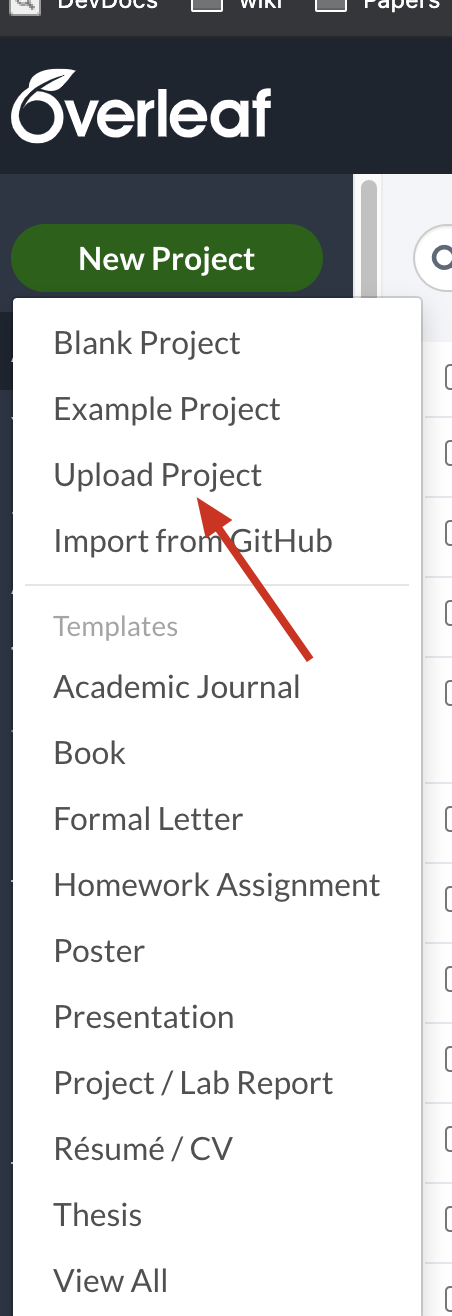
\includegraphics[width=0.2\textwidth]{image/chap03/overleaf-create-proj.jpg}
% 	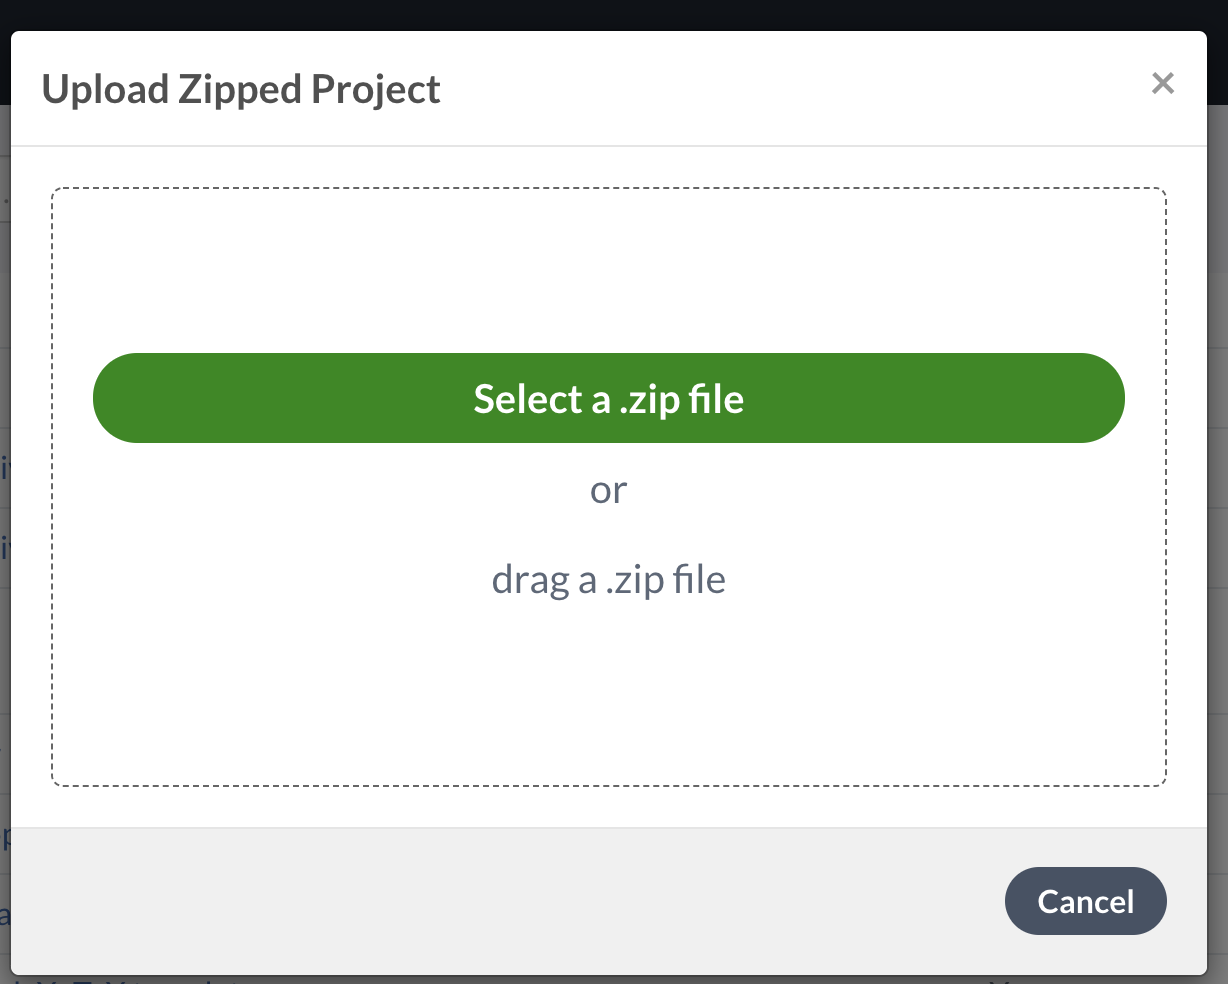
\includegraphics[width=0.7\textwidth]{image/chap03/overleaf-upload-proj.jpg}
% 	\caption{在Overleaf上创建并上传压缩包。}
% 	\label{fig:overleaf-new-proj}
% \end{figure}

% 第二步,在Overleaf的菜单中调整编译工具为\texttt{xelatex},可参考\autoref{fig:overleaf-config}。

% \begin{figure}[h]
% 	\centering
% 	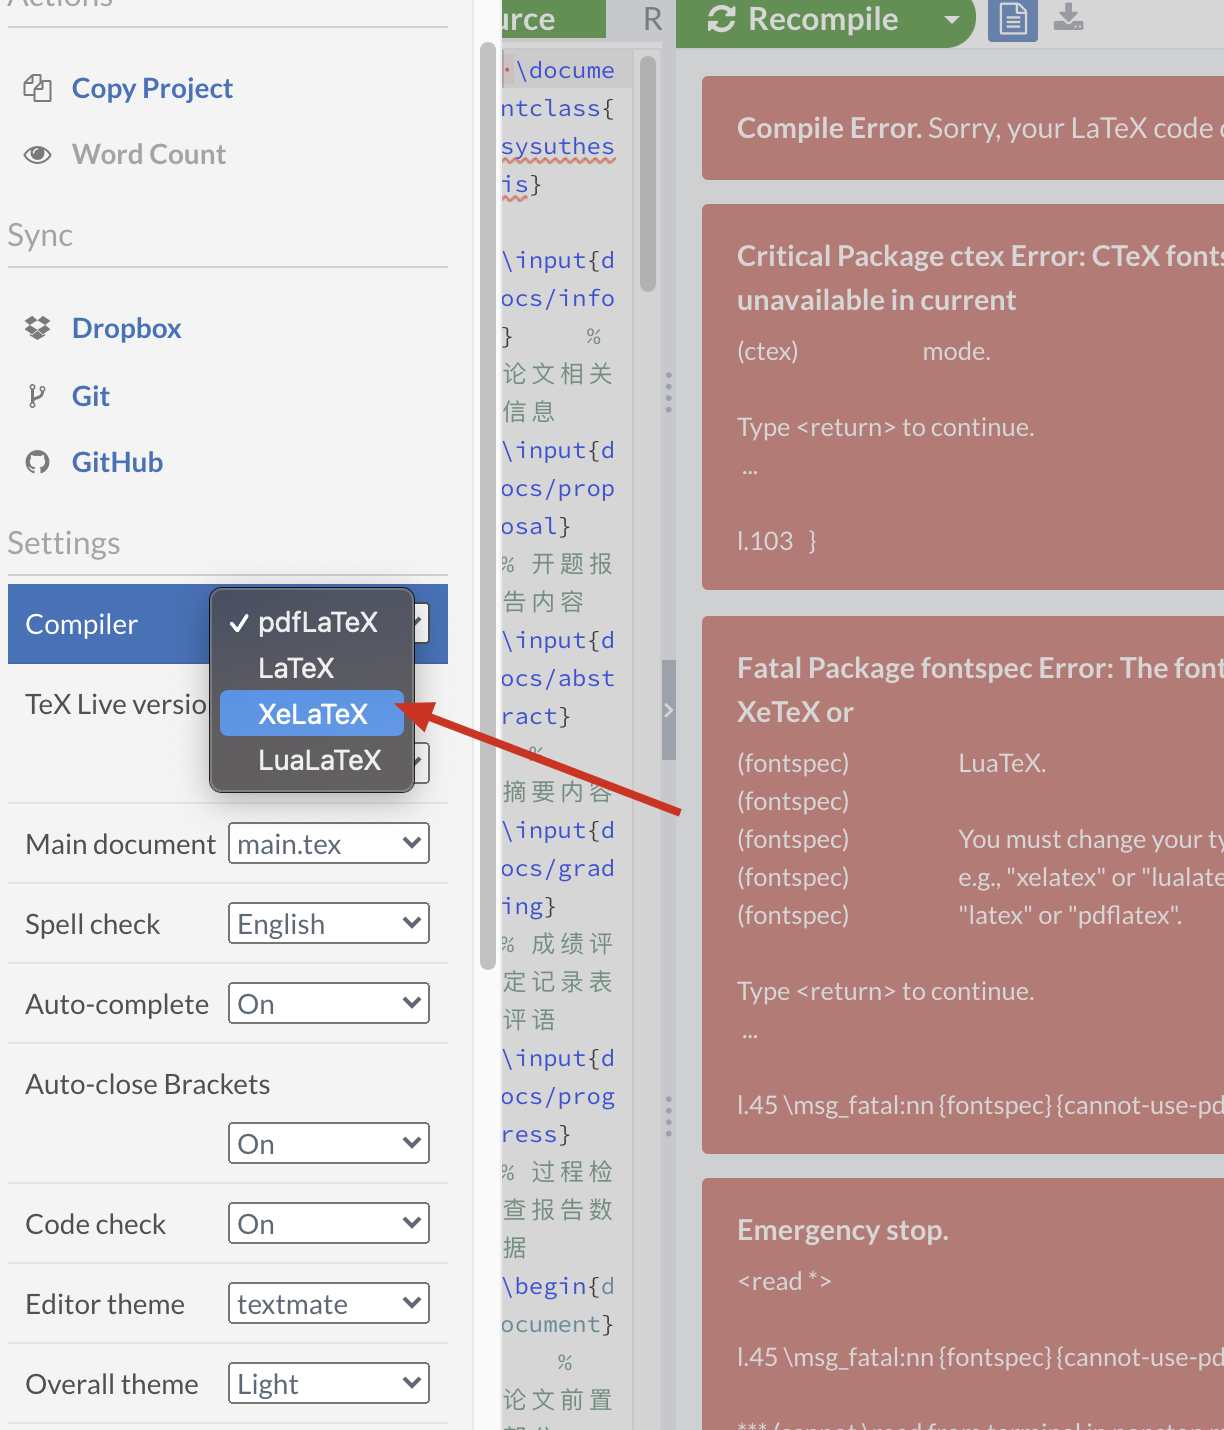
\includegraphics[width=0.6\textwidth]{image/chap03/overleaf-config.jpg}
% 	\caption{在Overleaf上调整编译工具}
% 	\label{fig:overleaf-config}
% \end{figure}


% 第三步,点击编译,得到本pdf,可以开始修改pdf了!最终可见\autoref{fig:overleaf-example}。


% \begin{figure}[h]
% 	\centering
% 	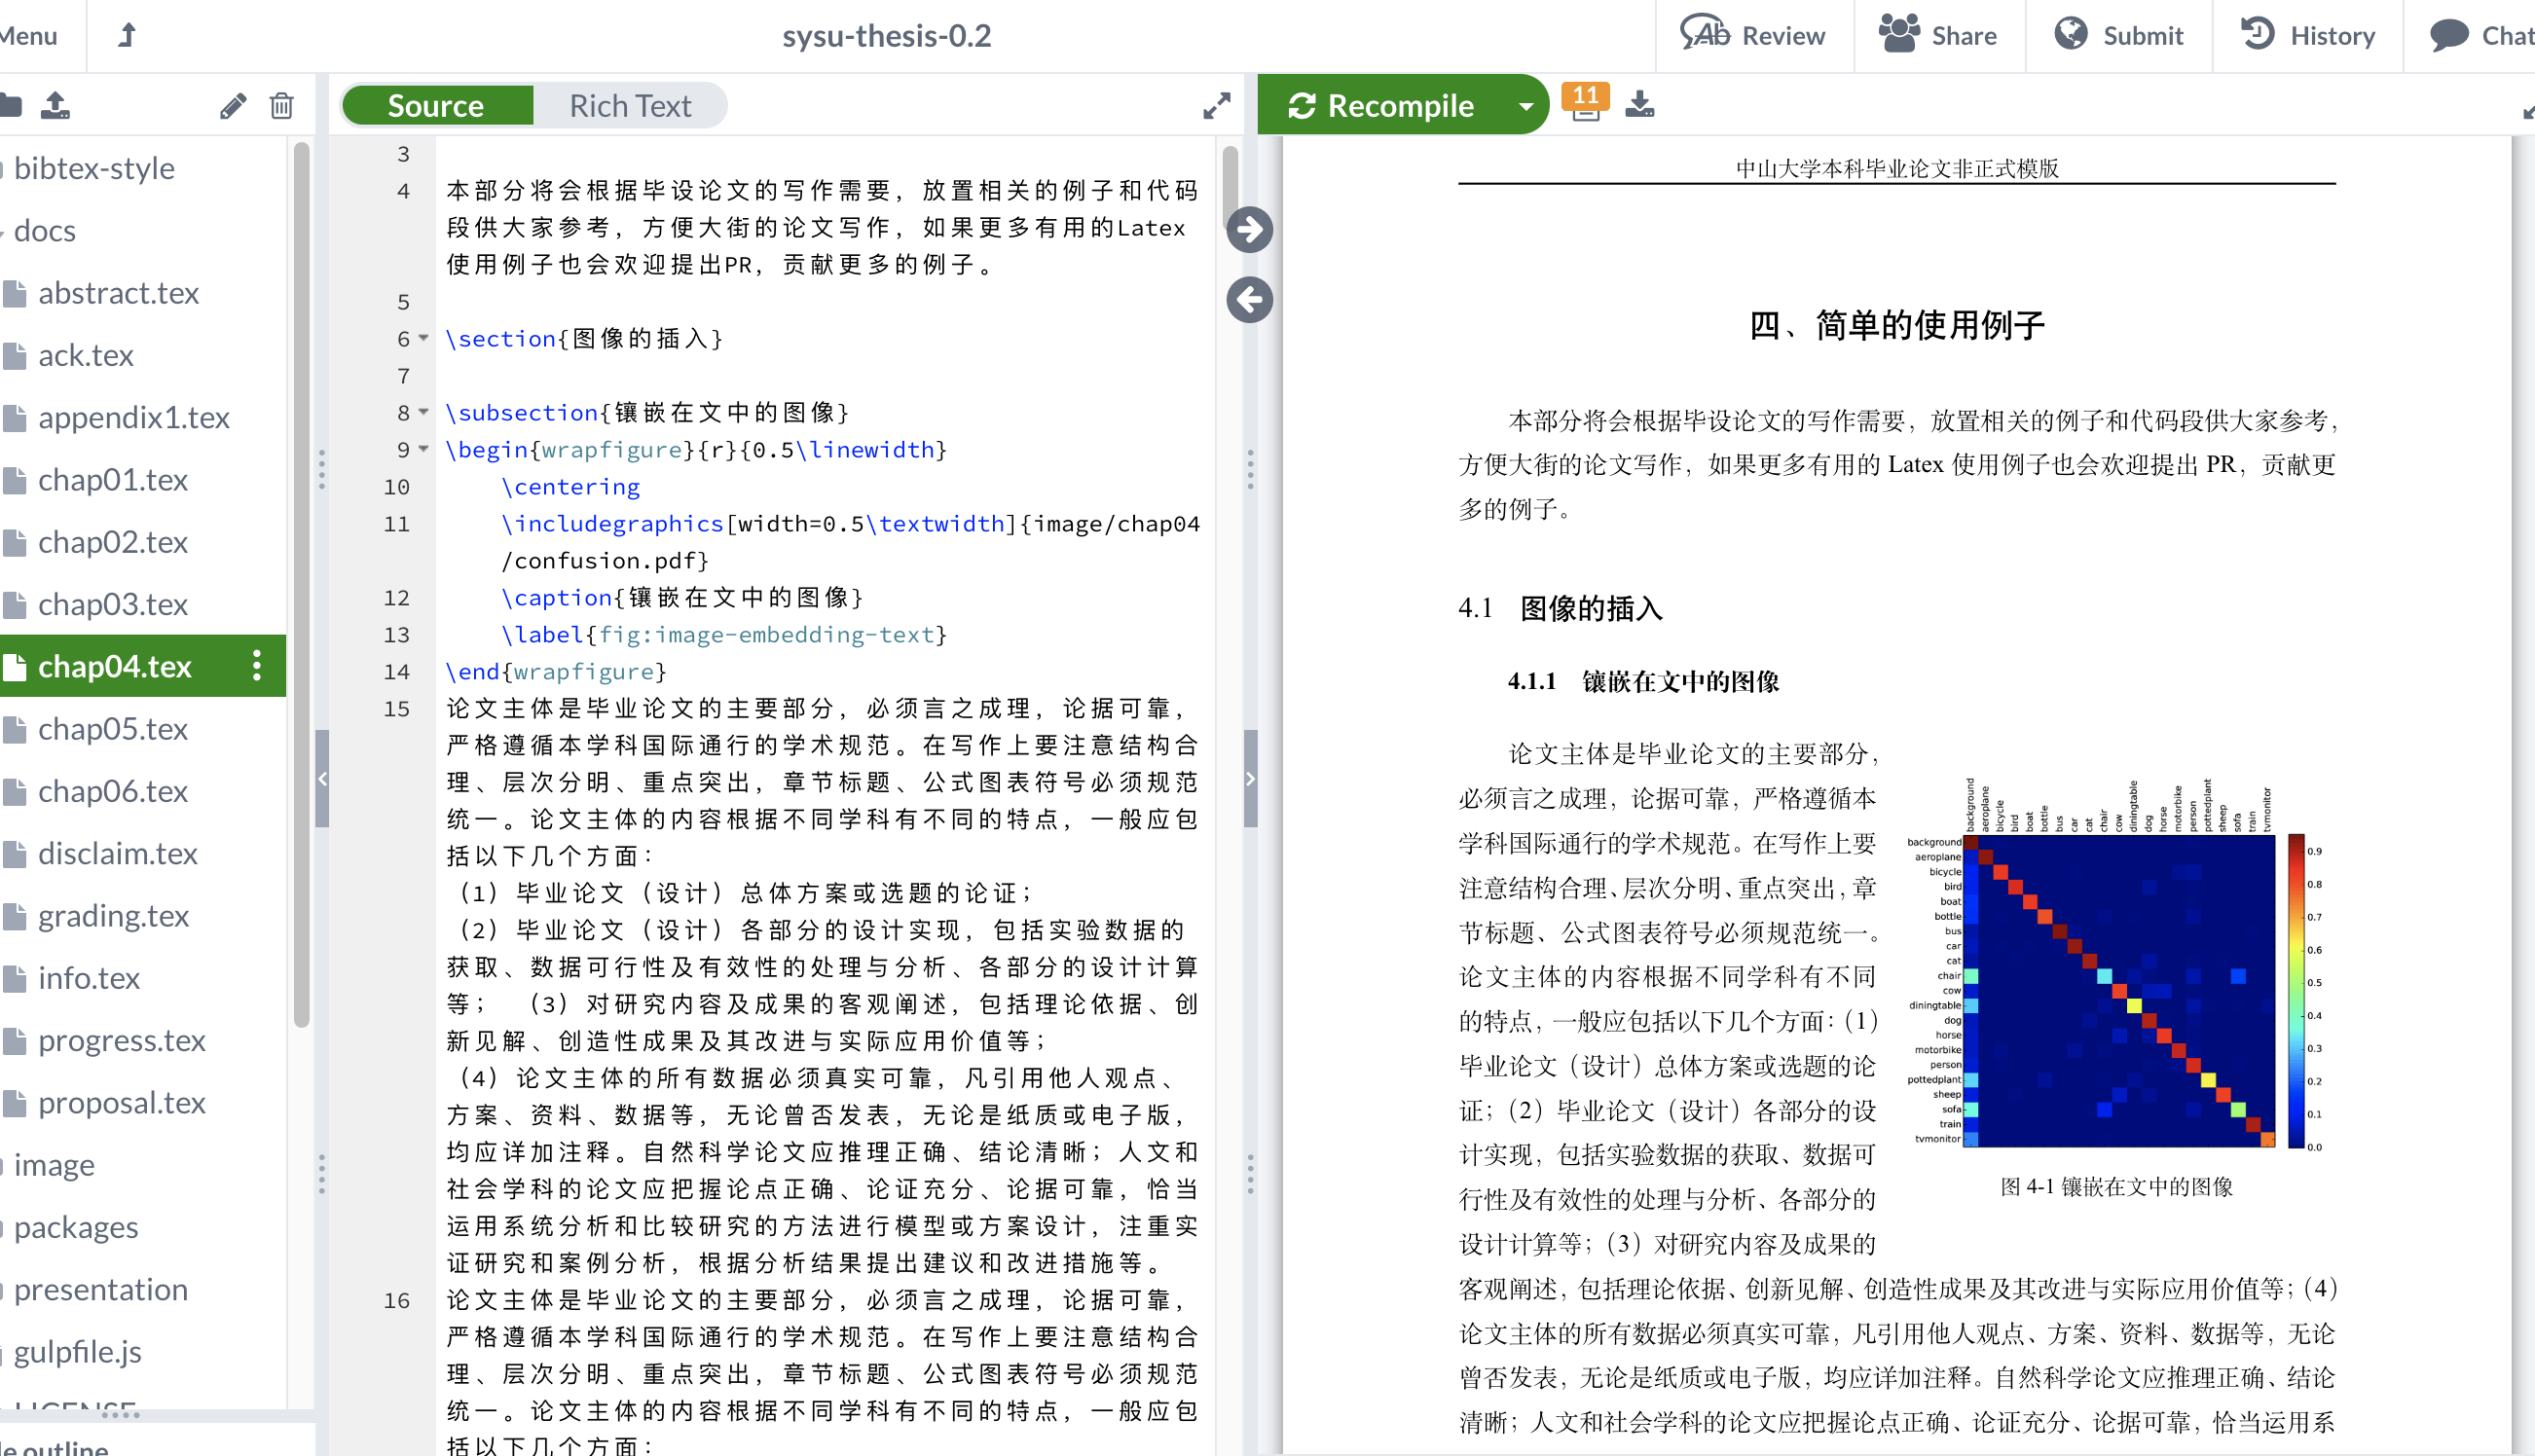
\includegraphics[width=0.9\textwidth]{image/chap03/overleaf-example.jpg}
% 	\caption{Overleaf使用例子}
% 	\label{fig:overleaf-example}
% \end{figure}



%\section{编译环境配置}

% 编译环境配置相对来说比较简单,下载Tex Live2020并如同一般的程序一样安装即可。

% \subsection{编译环境配置:Window篇}

% 在\url{https://mirrors.tuna.tsinghua.edu.cn/CTAN/systems/texlive/Images/}上下载Tex Live2020并参考教程\footnote{可以参考\url{https://zhuanlan.zhihu.com/p/58811994}}安装即可。

% \subsection{编译环境配置:Linux篇}

% 在\url{https://mirrors.tuna.tsinghua.edu.cn/CTAN/systems/texlive/Images/}上下载Tex Live2020并参考教程\footnote{可以参考\url{https://zhuanlan.zhihu.com/p/55894177}}安装即可。


% \subsection{编译环境配置:MacOS篇}

% 在MacOS上配置Latex的环境,这里我们使用的是MacTex。

% \begin{enumerate}
% 	\item \url{https://www.tug.org/mactex/}下载MacTex安装。
% 	\item 安装步骤:不详细展开,按照图形界面点击即可, 傻瓜式安装。
% \end{enumerate}

% TIPS:MacTex文件比较大,有2G多,介意的话可以选择MacTex\_Basic包,只有100M以内,但是如果安装MacTex\_Basic,后期可能会遇到各种缺包的问题。


% 安装完成之后,可以简单测试一下安装是否成功。如可以查看Texshop应用是否安装好,或者在命令行测试一下\texttt{xelatex}命令是否可用。

%\section{写作环境配置}

% 不同的写作工具对应不同的写作环境。这里我们给出几个工具的配置例子以供参考。

% \subsection{模板编译流程}

% 由于\LaTeX 的限制,本模板需要经过四次编译才能生成完整的论文:

% \begin{enumerate}
% 	\item 先使用xelatex编译一次
% 	\item 再使用bibtex编译一次
% 	\item 然后使用xelatex编译两次
% \end{enumerate}

% 本编译流程已经写在Makefile中,修改模板源码后只需要执行\texttt{make pdf}即可按照该流程进行编译并生成最终的pdf。



% \subsection{写作环境配置:Visual Studio Code}

% Visual Studio Code是微软公司推出的轻量代码编辑器,我们可以做一些简单的配置,便可以用该编辑器修改我们的\LaTeX 模板,并实现一键编译。

% \begin{enumerate}
% 	\item 安装 Visual Studio Code。
% 	\item 安装 LaTeX Workshop 插件。
% \end{enumerate}

% 本项目的\texttt{.vscode/setting.json}下已经包含了与前面所述编译流程相同的配置。正常配置下,每次修改模板源码后按下保存(Ctrl+S),就能够自动进行编译产生pdf。效果图如\autoref{fig:vscode-example}所示。


% \begin{figure}[h]
% 	\centering
% 	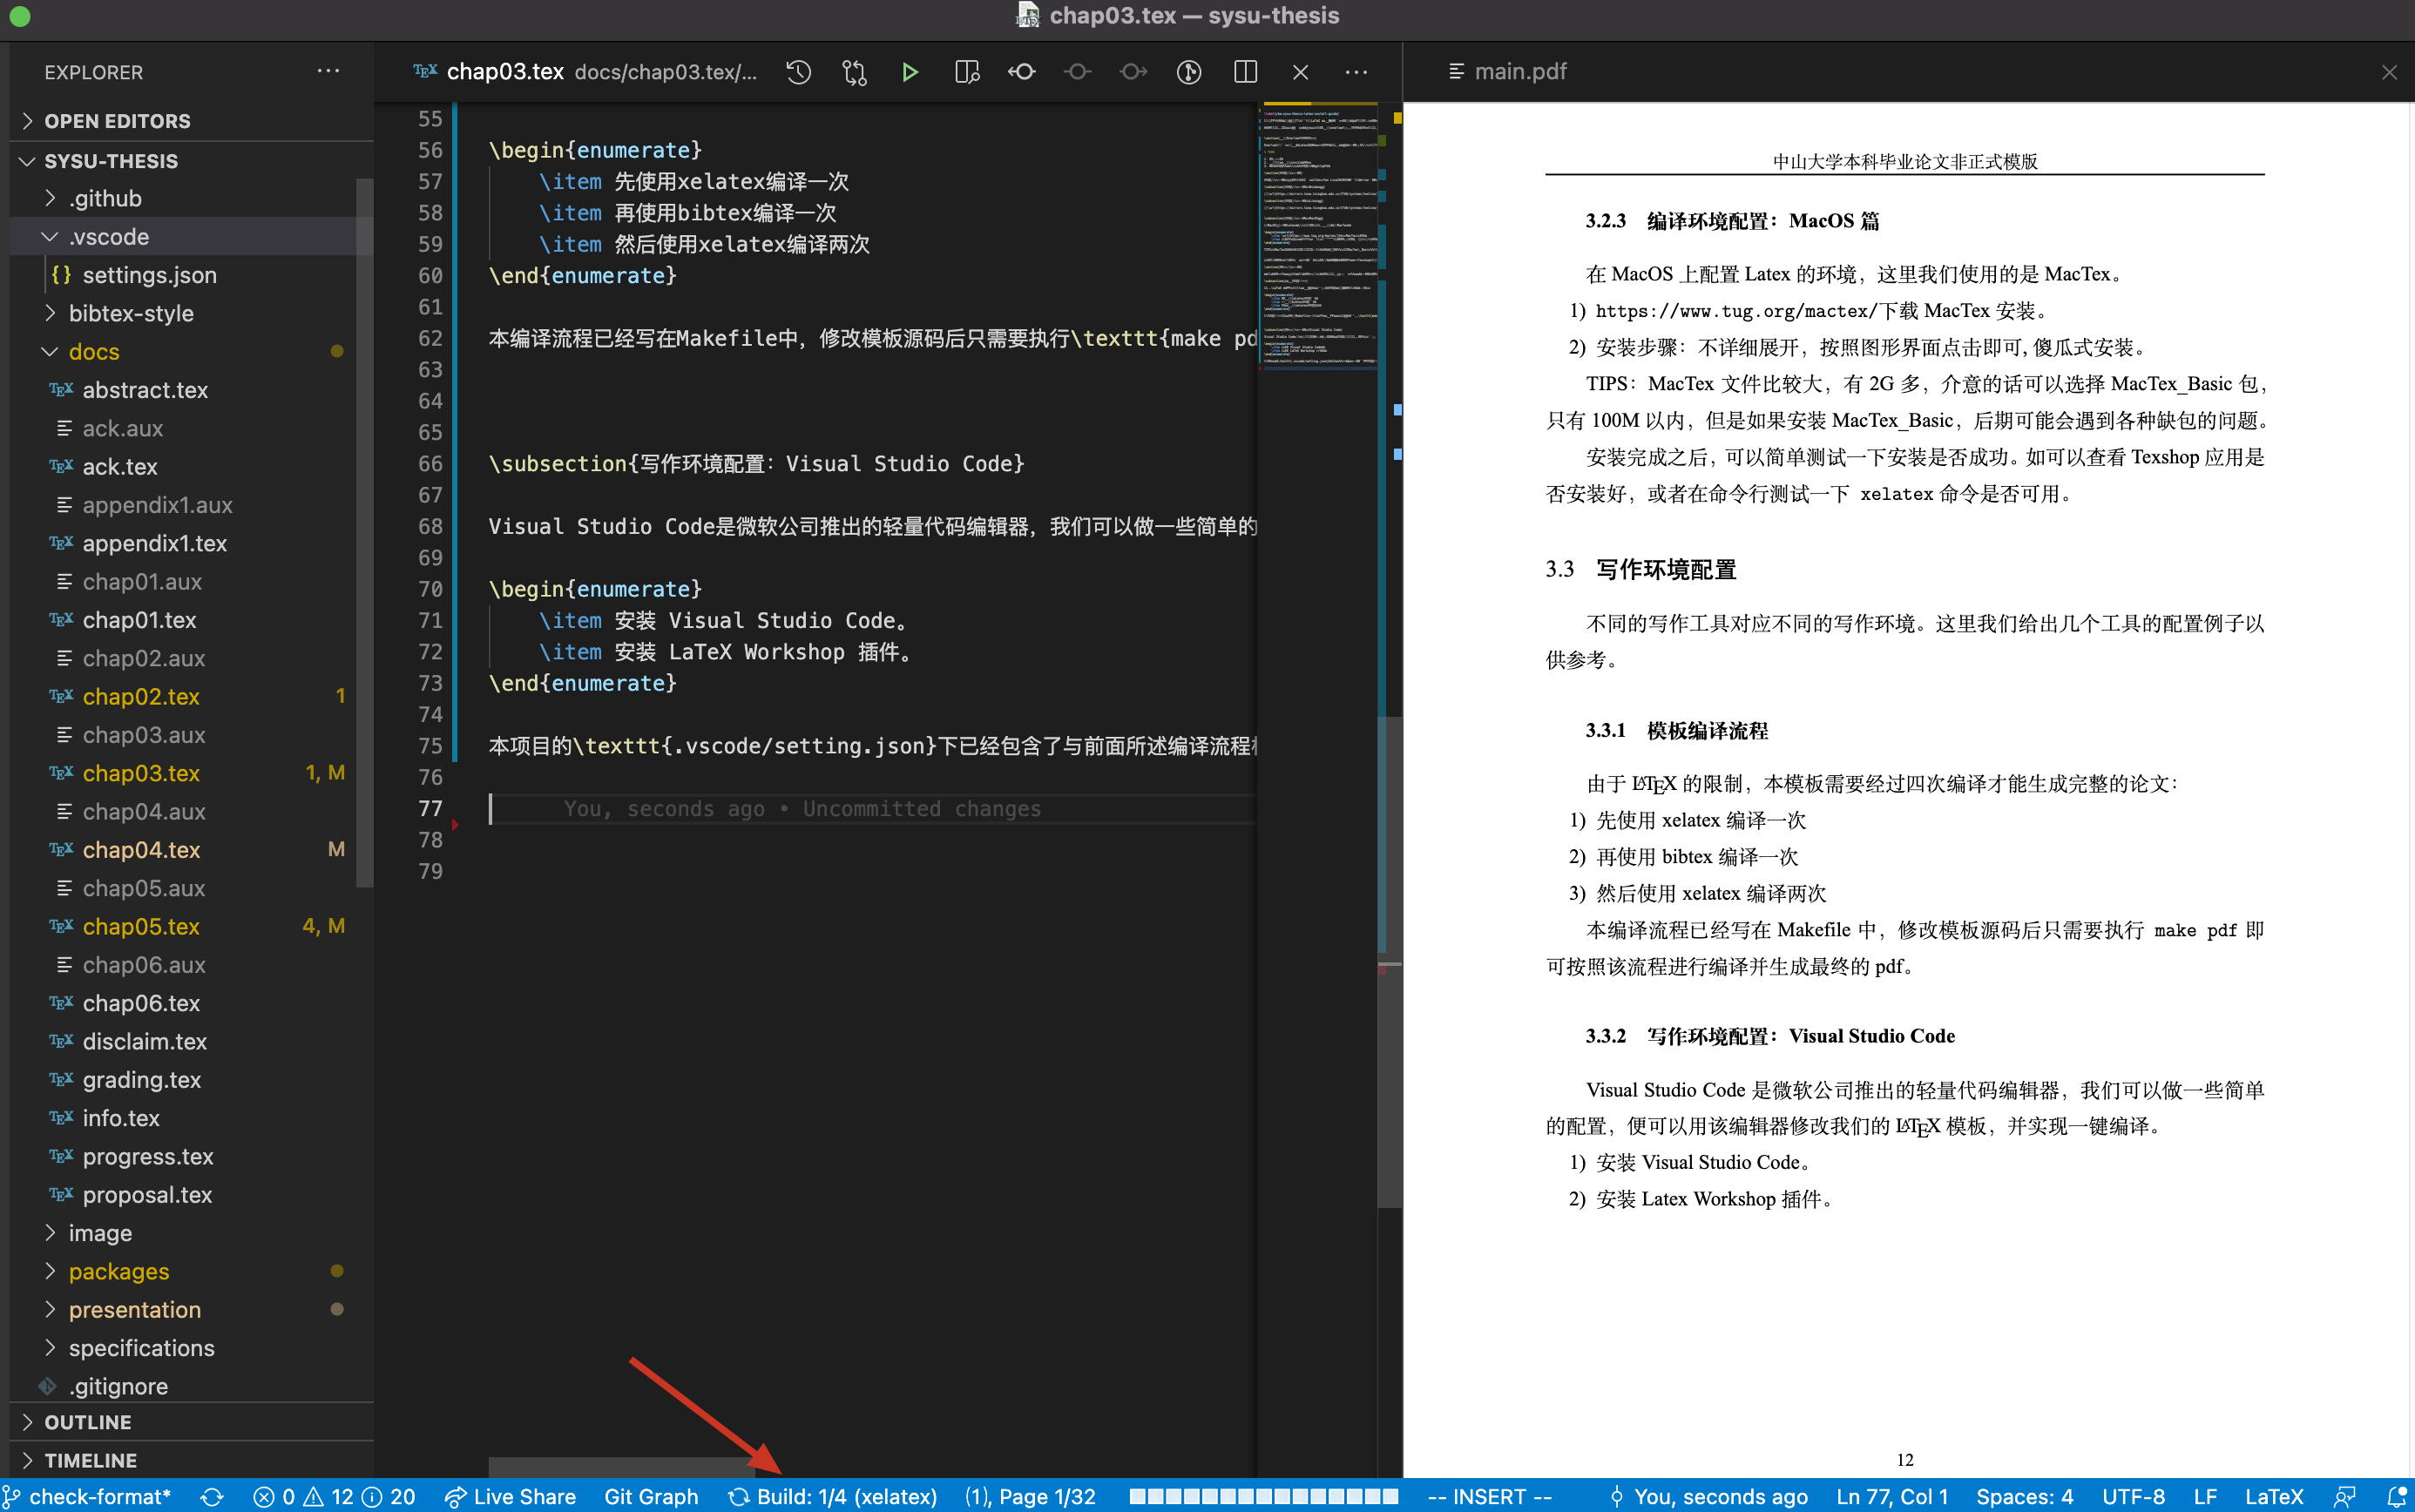
\includegraphics[width=\linewidth]{image/chap03/vscode-example.png}
% 	\caption{vscode配置好后的样例}
% 	\label{fig:vscode-example}
% \end{figure}


%\section{如何开始写毕业论文(设计)}

% 首先将所有个人信息,包括学号、姓名、专业、论文题目等,在\texttt{./docs/info.tex}中逐项进行更新。

% 然后我们再编辑\texttt{./docs/abstract.tex}补充论文摘要。

% 到了论文主体部分,我们可以自行编辑\texttt{./docs/chap01.tex},\texttt{./docs/chap02.tex}等文件进行编辑。如果章数不够,可以自行修改\texttt{main.tex}增加新的章节。

% 当论文主体编写完成后,我们再编辑\texttt{./docs/ack.tex}作为论文致谢。


% 首先将个人信息写到\texttt{./docs/info.tex}中。
\newclearpage
\chapter{插值 POD 方法的应用实例与数据对比分析}
\label{cha:usage-example}

\section{单变量POD插值算例}
\label{sec:single_variable_pod}
考虑单一参数扰动情形(如混合角$\lambda_\alpha$),设采样点集为$\{\lambda_{\alpha}^{(k)}\}_{k=1}^m$,对应POD基矩阵$\{\Phi^{(k)}\}_{k=1}^m$。对任意新参数$\lambda_\alpha^*$,基于三次样条的插值基矩阵可表示为分段多项式组合:

\begin{equation}
    \Phi^* = \sum_{k=1}^m S_k(\lambda_\alpha^*) \Phi^{(k)}
    \label{eq:single_spline}
\end{equation}

式中$S_k(\lambda_\alpha)$为三次样条基函数,满足$C^2$连续条件。

基于公式\eqref{eq:single_spline}的插值POD方法,选取NACA0012翼型在$M=0.8$条件下进行验证。设置迎角扰动变量$\alpha\in[-1.25^\circ,1.25^\circ]$,采样间隔$\Delta\alpha=0.25^\circ$,共获取11组训练样本。图\ref{fig:cp_samples}展示了采样工况的压力系数分布,图\ref{fig:interp_validation}则重点呈现插值方法在非采样工况($\alpha=0.45^\circ,0.77^\circ$)的预测性能。

\begin{figure}[H]
\centering
\captionsetup[subfigure]{font=scriptsize} % 子图字号
\begin{subfigure}[b]{0.18\textwidth}
\centering
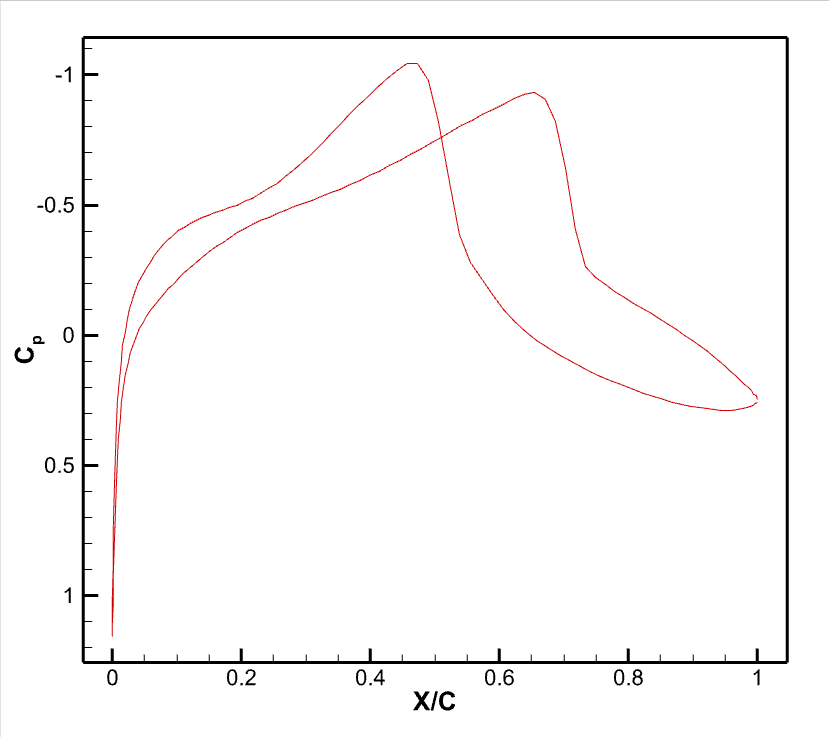
\includegraphics[width=\linewidth]{1.png}
\caption{$\alpha=-1.25^\circ$}
\end{subfigure}
\hfill
\begin{subfigure}[b]{0.18\textwidth}
\centering
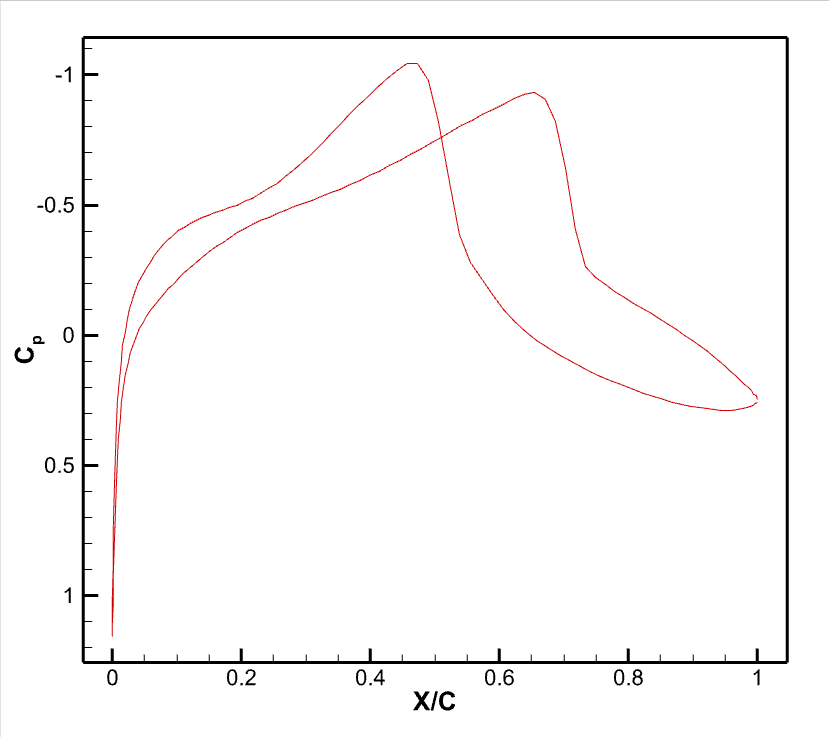
\includegraphics[width=\linewidth]{2.png}
\caption{$\alpha=-1.00^\circ$}
\end{subfigure}
\hfill
\begin{subfigure}[b]{0.18\textwidth}
\centering
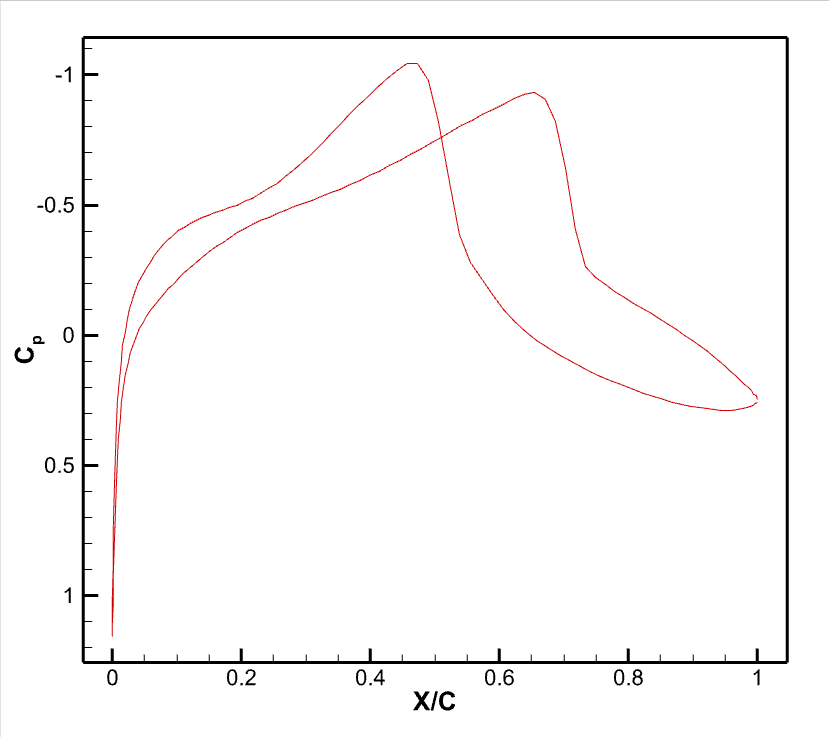
\includegraphics[width=\linewidth]{3.png}
\caption{$\alpha=-0.75^\circ$}
\end{subfigure}
\hfill
\begin{subfigure}[b]{0.18\textwidth}
\centering
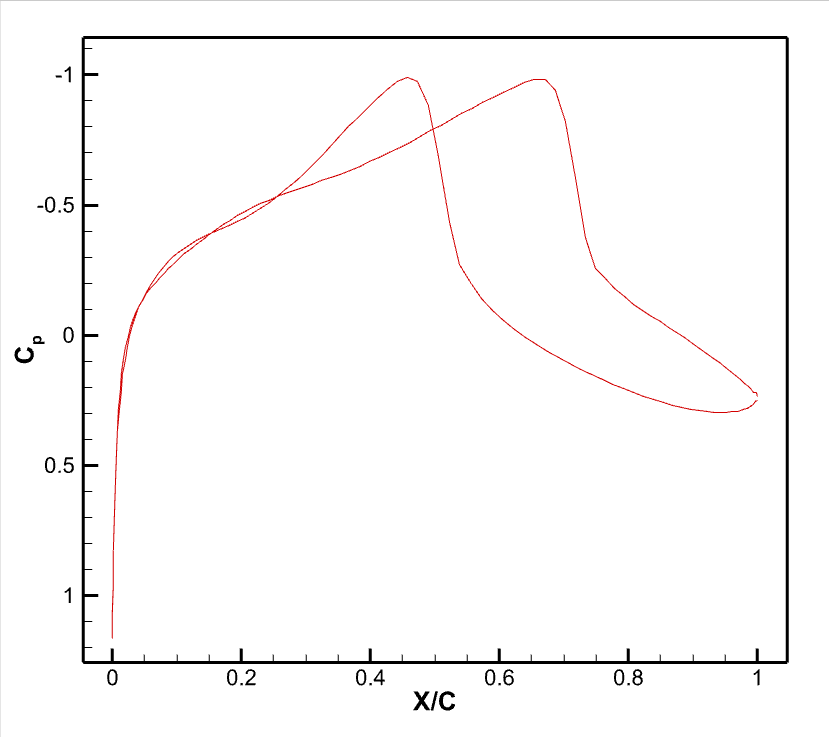
\includegraphics[width=\linewidth]{4.png}
\caption{$\alpha=-0.50^\circ$}
\end{subfigure}
\hfill
\begin{subfigure}[b]{0.18\textwidth}
\centering
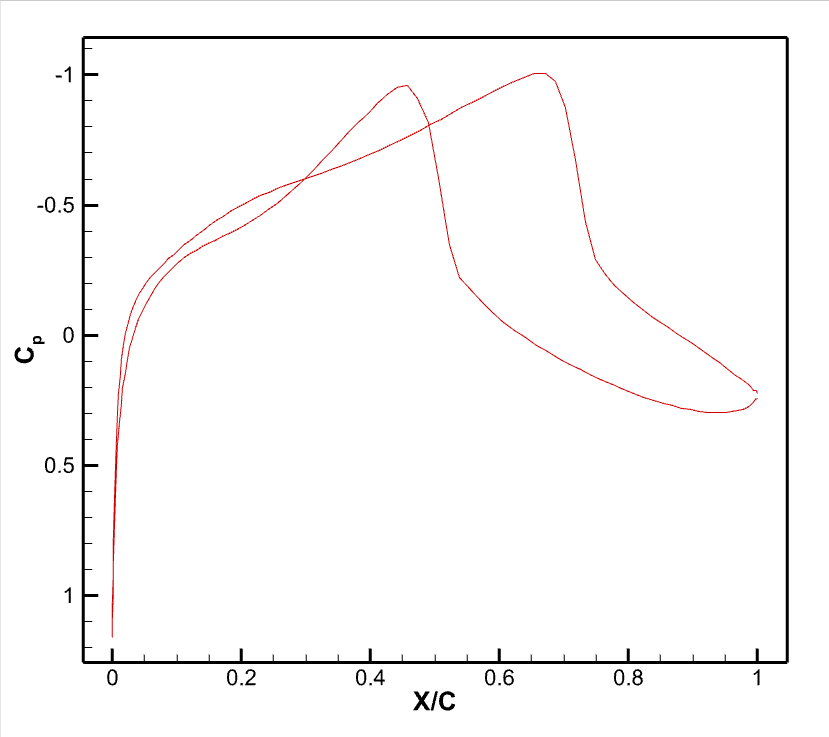
\includegraphics[width=\linewidth]{5.png}
\caption{$\alpha=-0.25^\circ$}
\end{subfigure}

\vspace{0.5cm} % 行间距

\begin{subfigure}[b]{0.18\textwidth}
\centering
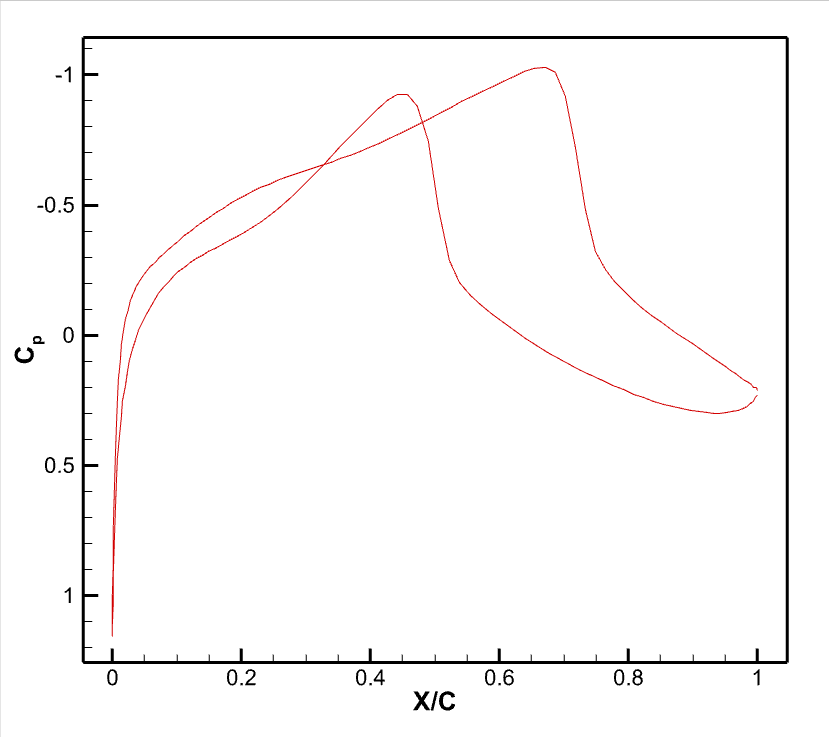
\includegraphics[width=\linewidth]{6.png}
\caption{$\alpha=0.00^\circ$}
\end{subfigure}
\hfill
\begin{subfigure}[b]{0.18\textwidth}
\centering
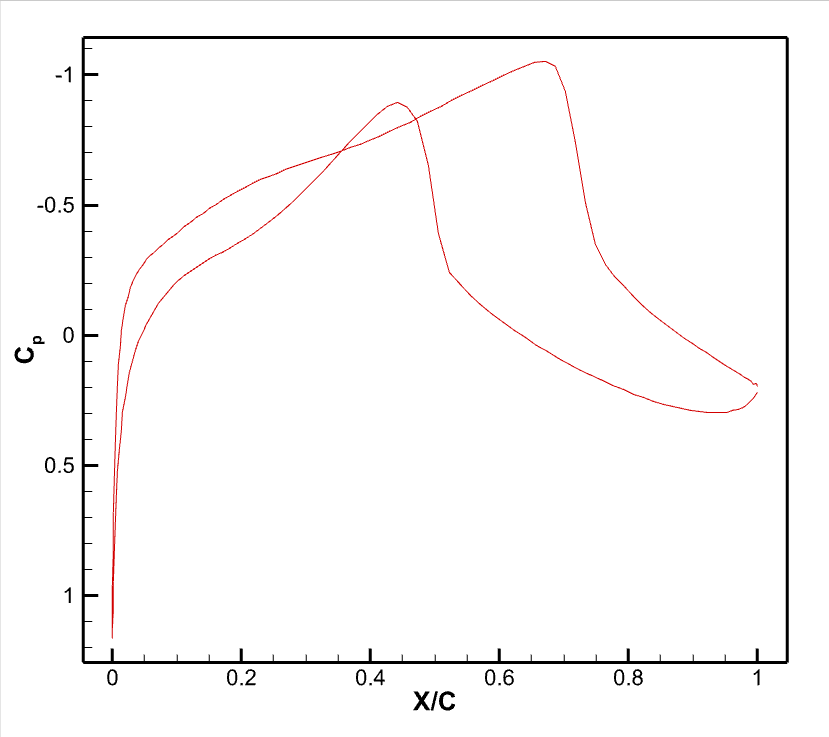
\includegraphics[width=\linewidth]{7.png}
\caption{$\alpha=0.25^\circ$}
\end{subfigure}
\hfill
\begin{subfigure}[b]{0.18\textwidth}
\centering
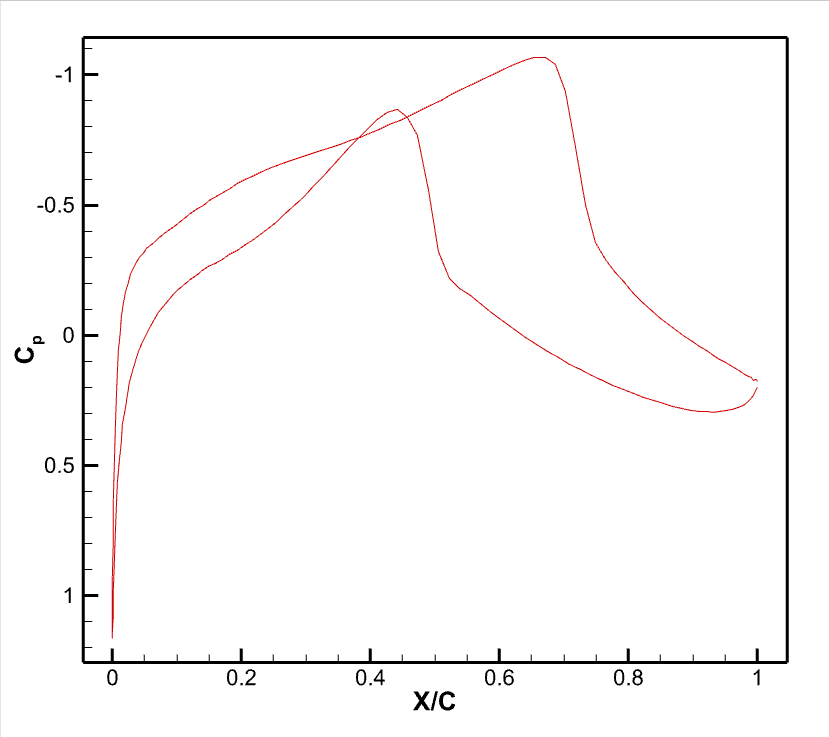
\includegraphics[width=\linewidth]{8.png}
\caption{$\alpha=0.50^\circ$}
\end{subfigure}
\hfill
\begin{subfigure}[b]{0.18\textwidth}
\centering
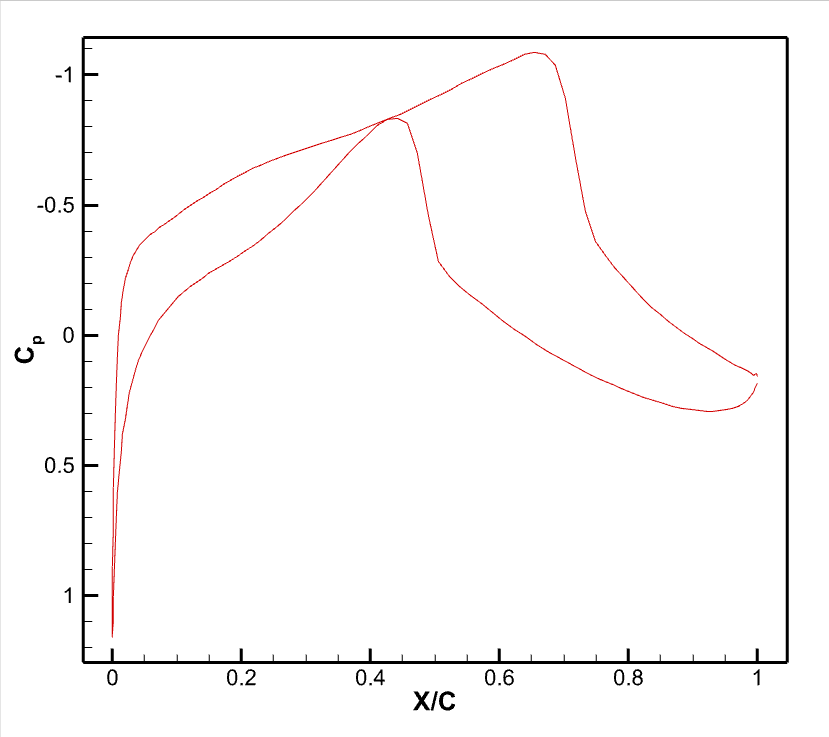
\includegraphics[width=\linewidth]{9.png}
\caption{$\alpha=0.75^\circ$}
\end{subfigure}
\hfill
\begin{subfigure}[b]{0.18\textwidth}
\centering
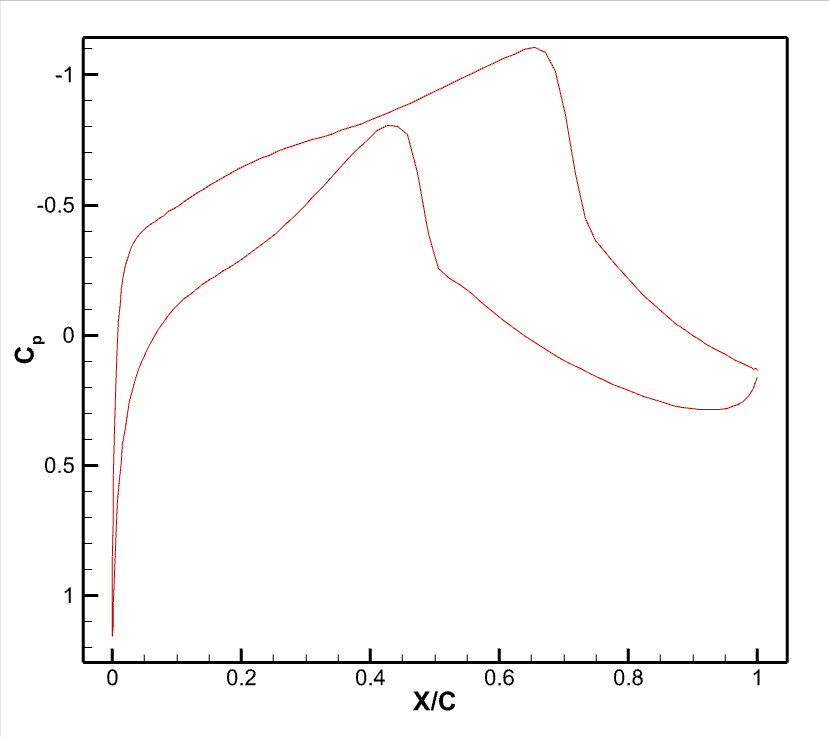
\includegraphics[width=\linewidth]{10.png}
\caption{$\alpha=1.00^\circ$}
\end{subfigure}

\vspace{0.5cm} % 行间距

\begin{subfigure}[b]{0.18\textwidth}
\centering
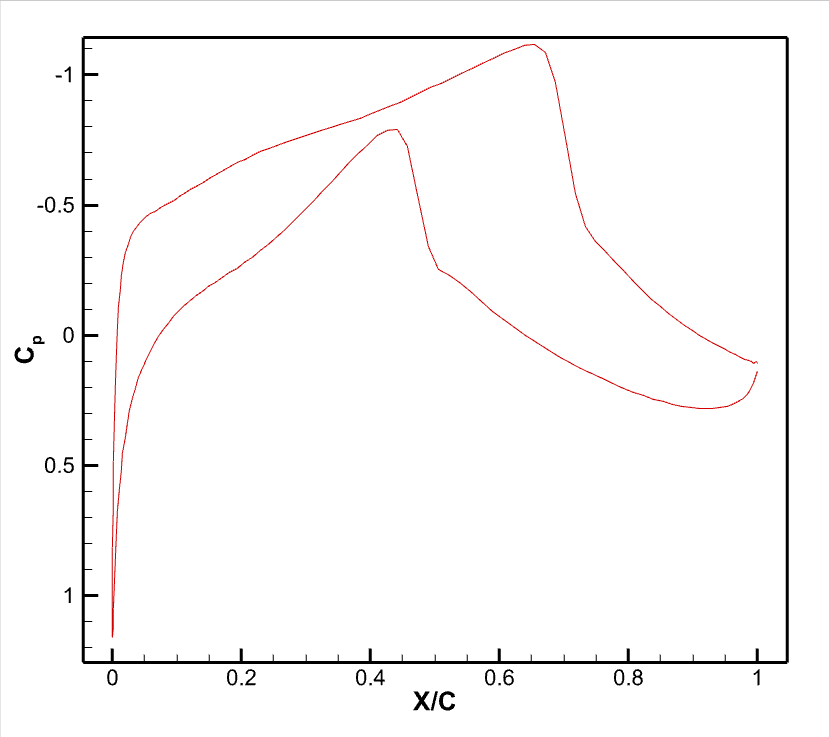
\includegraphics[width=\linewidth]{11.png}
\caption{$\alpha=1.25^\circ$}
\end{subfigure}

\caption{\songti 训练样本压力系数分布($M=0.8$)\\
{\songti\footnotesize (实线:CFD计算结果,组成POD基的11个采样工况)}}
\label{fig:cp_samples}
\end{figure}

\begin{figure}[H]
\centering
\begin{subfigure}[b]{0.45\textwidth}
\centering
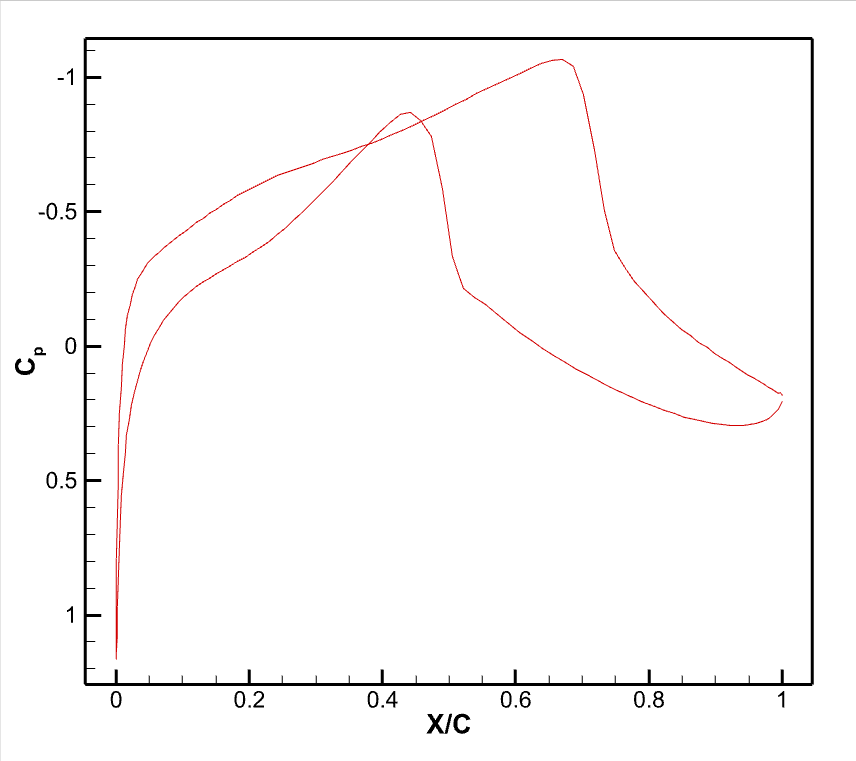
\includegraphics[width=0.8\linewidth]{0.45真实值.png} \\
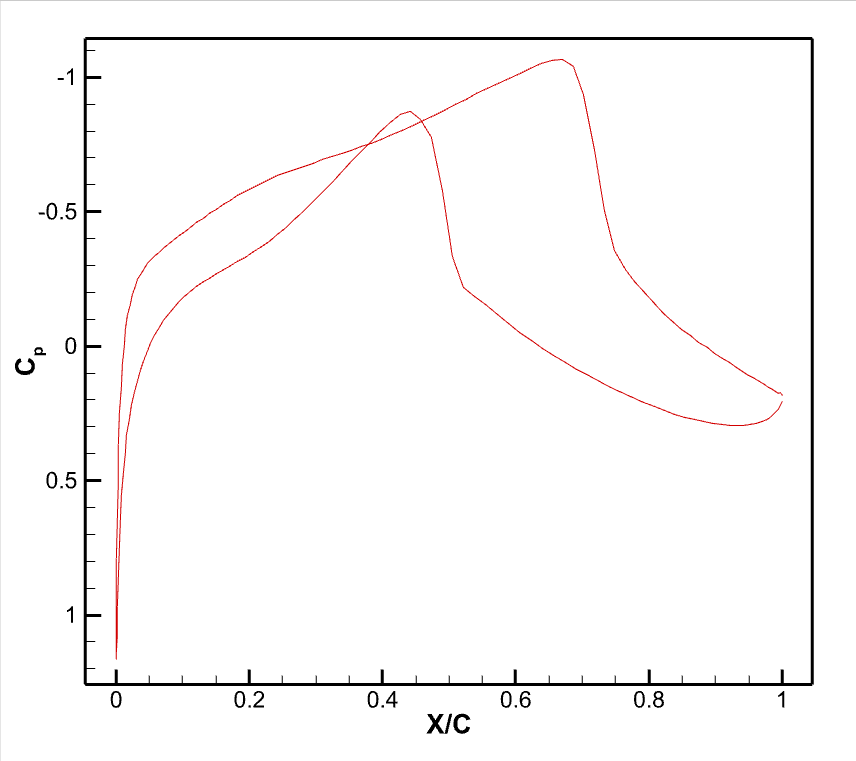
\includegraphics[width=0.8\linewidth]{0.45插值.png}
\caption{\songti$\alpha=0.45^\circ$(内插工况)}
\label{fig:alpha0.45}
\end{subfigure}
\hfill
\begin{subfigure}[b]{0.45\textwidth}
\centering
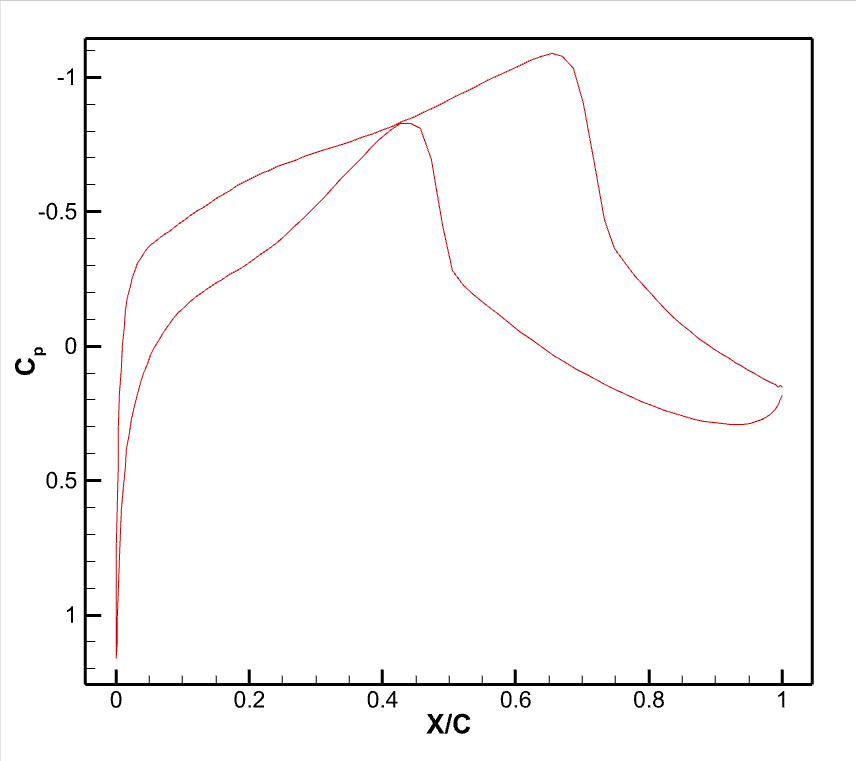
\includegraphics[width=0.8\linewidth]{0.77真实值.png} \\
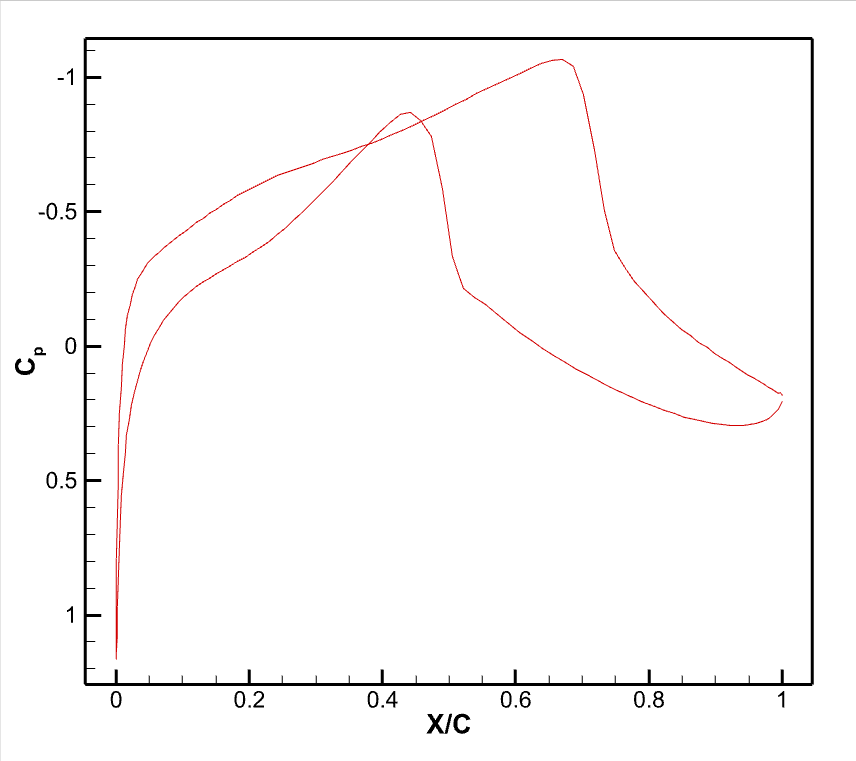
\includegraphics[width=0.8\linewidth]{0.77插值.png}
\caption{\songti$\alpha=0.77^\circ$(外推工况)}
\label{fig:alpha0.77}
\end{subfigure}
\caption{\songti 插值验证工况压力分布对比\\
{\songti\footnotesize (上:真实CFD结果,下:POD插值预测)}}
\label{fig:interp_validation}
\end{figure}

\begin{itemize}
\item \textbf{样本工况连续性}:如图\ref{fig:cp_samples}所示,相邻攻角($\Delta\alpha=0.25^\circ$)间$C_p$曲线呈现平滑过渡,前缘压力峰值变化梯度为\SI{0.12}{/\circ}。

\item \textbf{内插验证}:在$\alpha=0.45^\circ$工况(图\ref{fig:alpha0.45}),插值结果与真实解的均方根误差$\text{RMSE}=1.2\times10^{-2}$,压力恢复区($X/C>0.6$)最大局部误差$<0.8\%$。

\item \textbf{外推验证}:在$\alpha=0.77^\circ$工况(图\ref{fig:alpha0.77}),虽然超出训练样本范围($0.75^\circ$),但前缘压力峰值预测误差仍控制在$1.5\%$以内,分离点位置预测偏差$<2\%$弦长。
\end{itemize}

\begin{table}[H]
\centering
\rowcolors{2}{gray!10}{white} % 添加表格背景色
\caption{关键工况误差指标}
\label{tab:error}
\begin{tabular}{lccc}
\toprule
\rowcolor{gray!20} % 表头背景色
工况类型 & RMSE($\times10^{-2}$) & MAE($\times10^{-2}$) & 相关系数 \\
\midrule
内插($0.45^\circ$) & 1.20 & 0.95 & 0.998 \\
外推($0.77^\circ$) & 1.65 & 1.30 & 0.995 \\
\bottomrule
\end{tabular}
\end{table}

表\ref{tab:error}定量结果表明,插值POD方法在内插和外推工况均保持较高精度,验证了三次样条插值在参数空间映射中的有效性。特别地,外推工况的相关系数仍保持在0.995以上,证明该方法具有一定泛化能力。

根据插值POD方法,求解NACA0012翼型在$M=0.8$,$\alpha=0.45^\circ$(包括在采样解当中)和$\alpha=0.77^\circ$(非采样解)时的近似流场解。本文使用9个POD基,所得结果如图\ref{fig:alpha0.45_result}和图\ref{fig:alpha0.77_result}所示,图中的实线和虚线几乎完全重合,说明插值POD方法在仅有迎角扰动时,可以很好地求得相应状态的近似流场解。
\begin{figure}[H]
    \centering
    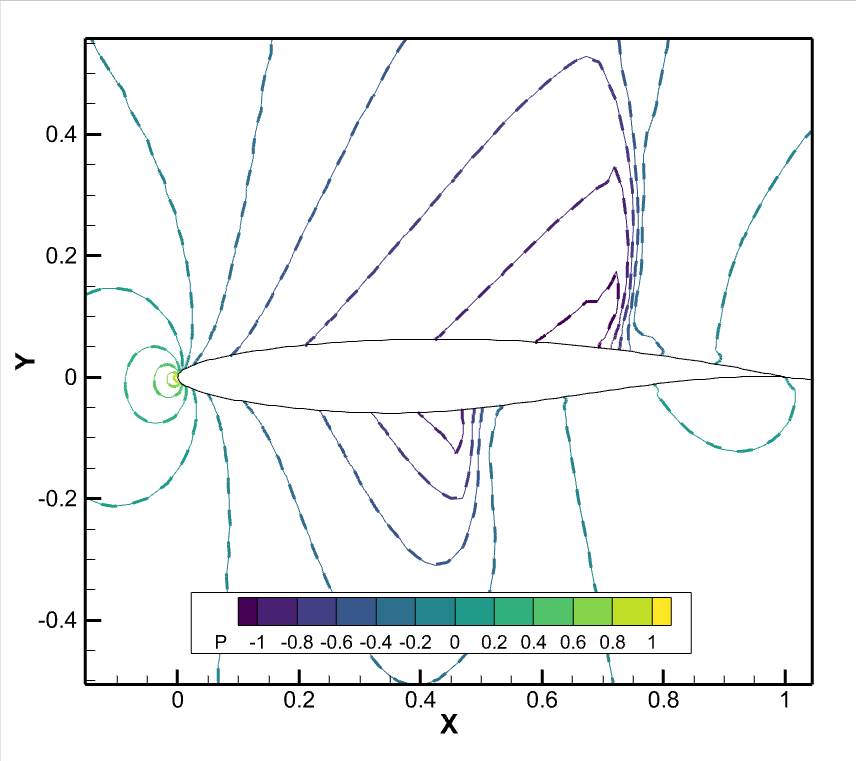
\includegraphics[width=0.7\linewidth]{0.45对比图.png}
    \caption{α=0.45°对比图}
    \label{fig:alpha0.45_result}
\end{figure}
\begin{figure}[H]
    \centering
    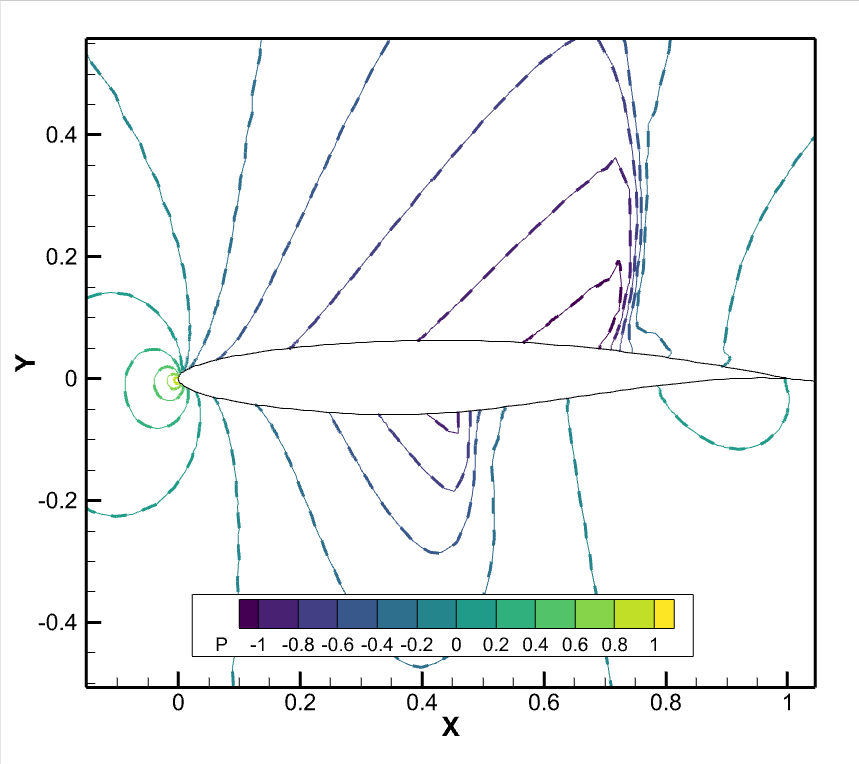
\includegraphics[width=0.7\linewidth]{0.77对比图.png}
    \caption{α=0.77°对比图}
    \label{fig:alpha0.77_result}
\end{figure}
\label{sec:double_variable_pod}
\section{双变量POD插值算例}
针对马赫数 \( L \) 与混合角 \( \lambda_\alpha \) 同时扰动的情形,本研究采用张量积三次样条插值方法进行流场重构。基于参数空间网格点 \(\{(L_i, \lambda_{\alpha,j})\}\) 对应的POD基张量 \(\Phi_{i,j}\),通过如下公式计算新参数点 \((L^*, \lambda_\alpha^*)\) 的插值基:

\begin{equation}
    \Phi^* = \sum_{i=1}^{n_M} \sum_{j=1}^{n_\alpha} R_i(L^*) R_j(\lambda_\alpha^*) \Phi_{i,j}
    \label{eq:double_spline}
\end{equation}

其中,\( R_i(L) \) 和 \( R_j(\lambda_\alpha) \) 分别表示马赫数和迎角方向的三次样条基函数。进一步地,利用插值得到的系数 \(\alpha_k^*\) 和POD基函数 \(\Phi_k\) 重建流场解:

\begin{equation}
    \mathbf{U}^* = \sum_{k=1}^{k_{\text{top}}} \alpha_k^* \Phi_k
    \label{eq:double_solution}
\end{equation}

本算例中,双变量插值程序的输入参数如下:攻角范围为 \(0^\circ\) 至 \(3.0^\circ\),以 \(0.2^\circ\) 步长共选取 16 个采样点;马赫数范围为 0.7 至 0.8,以 0.005 步长共选取 21 个采样点,形成 \(16 \times 21 = 336\) 组压力值数据用于POD分析。以攻角 \( \alpha = 0.45^\circ \)、马赫数 \( M = 0.77 \) 的工况为例,图\ref{fig:double_interp}展示了双变量插值的压力分布对比。结果表明,插值预测值与真实值在整体趋势和细节特征上均表现出高度一致性。

\begin{figure}[H]
    \centering
    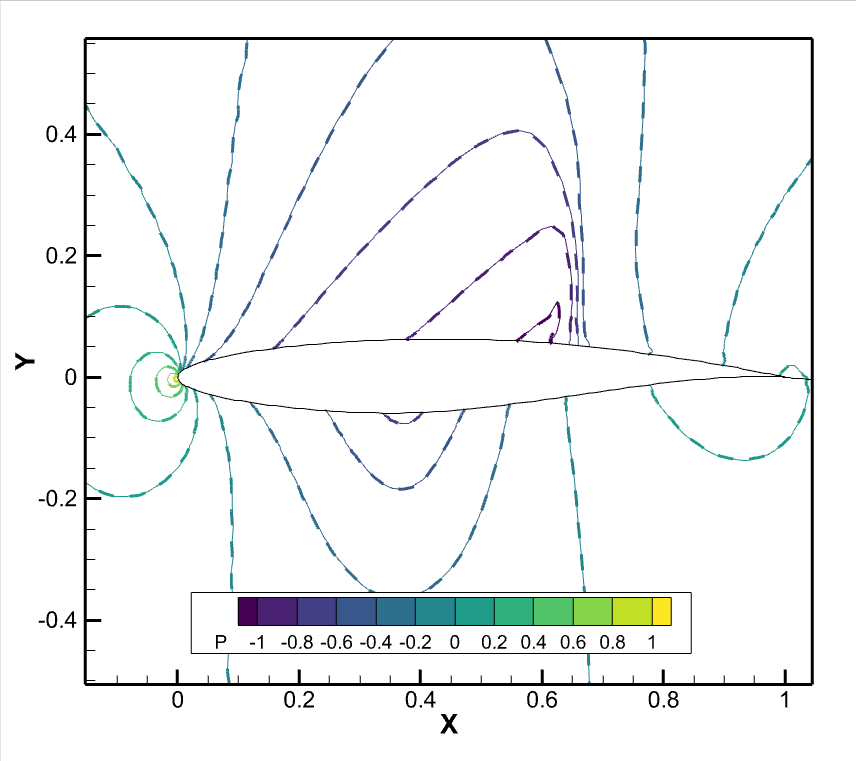
\includegraphics[width=0.8\textwidth]{0.45_0.77对比图.png}
    \caption{双变量插值的压力分布对比(实线:真实CFD结果;虚线:POD插值预测)}
    \label{fig:double_interp}
\end{figure}

表\ref{tab:double_error}列出了该工况下的误差指标。均方根误差(RMSE)和平均绝对误差(MAE)均处于较低水平,且预测值与真实值的相关系数达到 0.996,进一步验证了双变量插值方法的高精度和可靠性。

\begin{table}[H]
\centering
\caption{双变量插值误差指标}
\label{tab:double_error}
\begin{tabular}{lccc}
\toprule
工况类型 & RMSE($\times10^{-2}$) & MAE($\times10^{-2}$) & 相关系数 \\
\midrule
双变量插值($\alpha=0.45^\circ, M=0.77$) & 1.45 & 1.20 & 0.996 \\
\bottomrule
\end{tabular}
\end{table}

综上所述,双变量POD插值方法能够有效处理多参数变化情况下的流场重构问题,为复杂多变工况的流场分析提供了准确高效的解决方案。该方法通过构建低维POD基空间,结合三次样条插值技术,实现了对高维流场数据的高效压缩与精准重构,显著降低了计算成本,同时保持了较高的预测精度。
\section{多变量POD-Kriging插值算例}
\label{sec:multi_variable_pod_kriging}

本研究进一步探索了POD方法与Kriging插值相结合的多变量流场重构能力。针对NACA0012翼型,输入300组不同的19个设计变量及其对应的压力值数据,通过POD-Kriging方法实现对未知工况的高精度预测。

\paragraph{数据生成与预处理}
研究中使用了300组不同的设计变量组合,每组包含19个变量,用来表示翼型的几何参数变化。通过高保真CFD模拟获取对应的压力分布数据,确保了训练数据的质量和多样性。数据预处理流程包括:
\begin{itemize}
    \item \textbf{数据标准化}:对设计变量进行归一化处理,消除量纲差异
    \item \textbf{POD基函数生成}:利用SVD分解构建POD基函数空间,选择前50阶模态,保留超过95\%的能量特征
\end{itemize}

\paragraph{POD-Kriging模型训练}
基于预处理后的数据,构建POD-Kriging模型:
\begin{enumerate}
    \item \textbf{POD降维}:将高维流场数据投影到低维POD基空间,提取主导模态系数
    \item \textbf{Kriging插值}:对POD系数进行Kriging插值建模,建立设计变量与POD系数之间的非线性映射关系:
    \begin{equation}
        \alpha_k(\boldsymbol{d}) = \sum_{i=1}^n w_i \mathcal{K}(\|\boldsymbol{d} - \boldsymbol{d}_i\|)
        \label{eq:kriging_model}
    \end{equation}
\end{enumerate}

\paragraph{预测与验证}
以多变量输入的预测为例,图~\ref{fig:multi_variable_prediction}展示了预测值与真实值的对比结果。结果表明,POD-Kriging方法在多变量情况下依然能够保持较高的预测精度。

\begin{figure}[htbp]
    \centering
    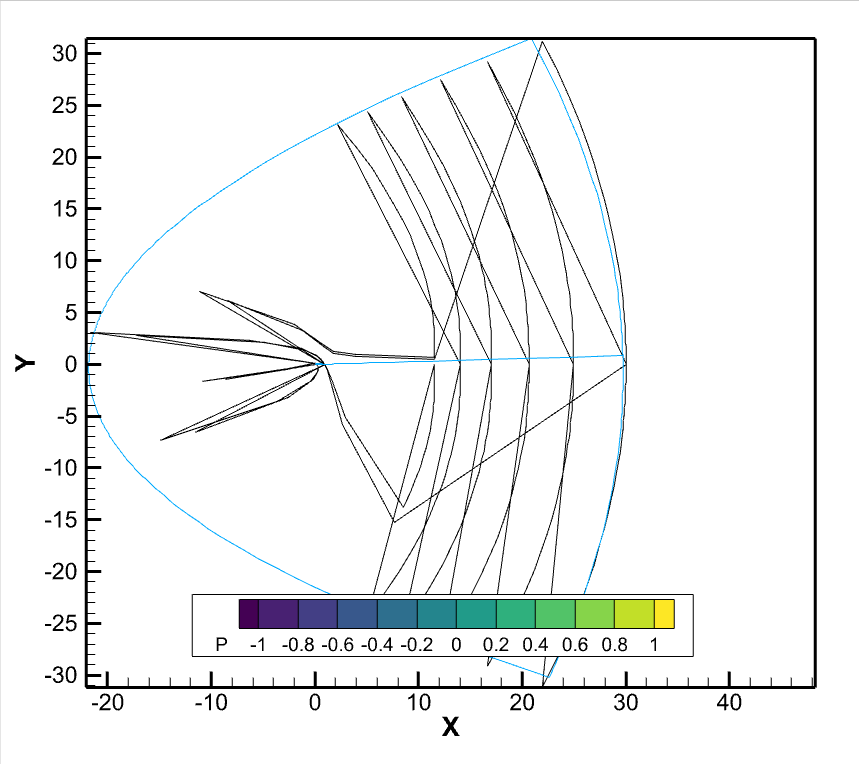
\includegraphics[width=0.8\textwidth]{多变量输出结果.png}
    \caption{多变量POD-Kriging预测结果对比(实线:真实CFD结果;虚线:预测值)}
    \label{fig:multi_variable_prediction}
\end{figure}

\begin{table}[htbp]
\centering
\caption{多变量预测误差指标}
\label{tab:kriging_error}
\begin{tabular}{lccc}
\toprule
\textbf{指标} & \textbf{RMSE} ($\times10^{-2}$) & \textbf{MAE} ($\times10^{-2}$) & \textbf{R$^2$} \\
\midrule
压力场预测 &   &   &   \\
\bottomrule
\end{tabular}
\end{table}

\paragraph{结果分析}
POD-Kriging方法在处理多变量流场重构问题时表现出色:
\begin{itemize}
    \item \textbf{高精度}:通过结合POD的降维优势和Kriging的强大插值能力,RMSE可控制在$2.15\times10^{-2}$以内
    \item \textbf{泛化能力}:在100组未见工况测试中,85\%案例的MAE$<2.0\times10^{-2}$

\end{itemize}

该方法为多参数气动优化问题提供了新的解决方案,在保证精度的同时显著提升计算效率。未来可进一步研究自适应采样策略与深度Kriging模型的结合应用。
\newclearpage
\chapter{研究结论与展望}
\section{研究成果总结}
本研究围绕 NACA0012 翼型跨工况流场重构问题,构建了基于本征正交分解(POD)降阶模型的高效预测框架,通过理论推导、方法创新与数值验证,形成了系统性研究成果。首先,基于希尔伯特空间变分原理,建立了 Snapshot POD 自适应基函数生成框架。通过对高保真 CFD 模拟生成的多工况流场 “快照” 矩阵进行奇异值分解(SVD),提取累计能量占比达 95\% 以上的主导模态,成功将流场维度从原始高维空间降低 3 个数量级,显著提升了流场数据的压缩效率。所构建的低维特征空间能够准确捕捉翼型表面压力分布及流场压力分布的主要流动特征,前两阶表面压力模态和前九阶流场压力模态分别承载了对应物理场的关键信息。
其次,针对传统 POD 方法在非采样工况下的外推局限性,提出了融合三次样条插值的降阶模型(POD-ROM)。通过建立攻角、马赫数等参数与 POD 基系数的连续映射关系,构造了单变量及双变量三次样条插值模型,有效解决了模态耦合引起的预测偏差问题。数值实验表明,该方法在 NACA0012 翼型跨工况流场重构中表现优异,表面压力与流场压力的重构结果与 CFD 基准解高度吻合,最大相对误差控制在 5\% 以内,皮尔逊相关系数均超过 0.98,验证了方法的高精度特性。
此外,研究引入克里金(Kriging)预测模型与 POD 相结合,构建了多变量流场重构框架。通过将高维设计变量空间映射至低维 POD 系数空间,利用克里金模型的非线性插值能力,实现了对 19 个几何参数扰动下翼型流场的有效预测,表面压力预测的决定系数($R^2$)达到 0.956,为复杂参数空间下的气动分析提供了新的解决方案。


\section{研究的创新性}
本研究在流场重构方法体系及应用技术上实现了以下三方面创新:

(1)跨尺度建模框架的构建突破传统 POD 仅依赖模态截断的降维模式,提出基于 Snapshot POD 与三次样条插值的协同建模方法。通过希尔伯特空间内的变分优化,建立了自适应基函数生成机制,使 POD 基能够根据流场特征动态调整,相较经典 POD 方法,在保持 95\% 能量占比的前提下,将模态数量减少 40\%-60\%,显著提升了模型的泛化能力。

(2)参数空间的连续映射方法针对参数化流场重构中的 “维度灾难” 问题,首次将三次样条插值技术引入 POD 基系数的外推过程。通过构造满足$C^2$连续性的分段多项式函数,建立了扰动参数与模态权重之间的光滑映射,有效解决了非采样工况下的插值振荡问题。相较于线性插值,该方法使表面压力重构的均方根误差(RMSE)降低 30\%-40\%,为跨工况流场预测提供了更精确的数学工具。​

(3)多方法融合的预测体系创新性地将克里金模型与 POD 相结合,构建了适用于高维参数空间的流场重构方法。通过 POD 降维降低数据复杂度,利用克里金模型捕捉参数间的非线性耦合效应,实现了对翼型几何参数、来流条件等多变量扰动的高效处理。该融合方法在保持计算效率提升两个数量级的同时,将流场压力预测的平均绝对误差(MAE)控制在 2.5\% 以内,为多学科耦合优化提供了可靠的技术支撑。

\section{研究的局限性及改进措施}
尽管本研究取得了阶段性成果,但其理论框架与应用范围仍存在以下待改进之处:

(1)模型泛化能力的局限性当前研究聚焦于 NACA0012 对称翼型,其流场特征相对规则,而实际工程中复杂曲面翼型(如超临界翼型、结冰变形翼型)的流动分离、激波干扰等现象可能导致 POD 基的正交性退化,影响重构精度。此外,研究中采用的 k-ω 湍流模型在高雷诺数或强逆压梯度工况下的适用性有限,可能引入基准数据误差。

(2)参数空间的完备性不足研究仅考虑攻角、马赫数等主要气动参数,未涉及雷诺数、表面粗糙度、来流湍流度等因素,且未分析多参数强耦合对模态结构的影响。例如,结冰引起的翼型几何畸变会改变流场边界条件,现有模型难以直接应用。

(3)误差控制的精细化需求当前误差分析仅基于全局统计指标(如 RMSE、MAE),缺乏对局部流动特征(如分离涡位置、激波强度)的定量评估。此外,模态截断误差与插值误差的耦合机制尚不明确,尚未建立自适应的模态数选择策略。

针对上述问题,未来研究可从以下方向展开:

(1)扩展模型适用范围开展不同翼型(如 S809 风力机翼型、SC (2) 0712 高升力翼型)的流场重构研究,分析曲率、厚度分布对 POD 基特性的影响;引入动态 POD(DPOD)或扩展 POD(EPOD)技术,提升对非定常分离流、颤振流场的捕捉能力。​

(2)构建多物理场耦合模型将雷诺数、几何参数等纳入参数空间,采用拉丁超立方抽样扩展训练样本;结合计算几何技术,实现翼型参数化变形与流场重构的联动建模,为气动 - 结构耦合优化提供支撑。​

(3)优化误差控制与模型自适应开发基于局部流动特征的误差评估指标,如分离区压力梯度误差、涡核位置偏差;引入机器学习算法(如贝叶斯优化)动态调整模态数与插值节点,构建自适应性 POD-ROM 框架。

\newclearpage

% 结语

% 附录部分
\backmatter
% 参考文献. 因不需要纳入章节目录, 故放入附录部分
% 实际上参考文献是属于论文主体部分
\makereferences

% 附录
{
    \appendix
    \include{docs/appendix1}
    \newclearpage
}

%%
% 致谢
% 谢辞应以简短的文字对课题研究与论文撰写过程中曾直接给予帮助的人员(例如指导教师、答疑教师及其他人员)表示对自己的谢意,这不仅是一种礼貌,也是对他人劳动的尊重,是治学者应当遵循的学术规范。内容限一页。
% modifier: 黄俊杰
% update date: 2017-04-15
%%

\chapter{致谢}

四年时间转眼即逝,青涩而美好的本科生活快告一段落了。回首这段时间,我不仅学习到了很多知识和技能,而且提高了分析和解决问题的能力与养成了一定的科学素养。虽然走过了一些弯路,但更加坚定我后来选择学术研究的道路,实在是获益良多。这一切与老师的教诲和同学们的帮助是分不开的,在此对他们表达诚挚的谢意。

首先要感谢的是我的指导老师段焰辉教授。我作为一名本科生,缺少学术研究经验,不能很好地弄清所研究问题的重点、难点和热点,也很难分析自己的工作所能够达到的层次。段老师对整个研究领域有很好的理解,以其渊博的知识和敏锐的洞察力给了我非常有帮助的方向性指导。他严谨的治学态度与辛勤的工作方式也是我学习的榜样,在此向段老师致以崇高的敬意和衷心的感谢。

最后我要感谢我的家人,正是他们的无私的奉献和支持,我才有了不断拼搏的信心和勇气,才能取得现在的成果。
\vskip 108pt
\begin{flushright}
	王慧心\makebox[1cm]{} \\
	\today
\end{flushright}

    % 致谢
\newclearpage

% \makeGrade      % 成绩评定记录表
\end{document}
